% !TeX root = ../main.tex
% !TeX program = xelatex
% !TeX encoding = UTF-8
\section{负荷预测与协同优化模型}\label{minor:model}

\subsection{基本假设}

为明确模型适用范围，作如下假设：
\begingroup
\setlength{\parskip}{0pt}
\newcommand{\assumptionline}[2]{\par\noindent\hangindent=1.8em\hangafter=1 #1.\hspace{0.5em}#2}
\assumptionline{1}{研究区域由热源节点、管网节点、换热站和典型建筑构成，同类建筑在保持负荷特征的前提下聚合处理；}
\assumptionline{2}{气象、建筑参数、设备性能和能源价格按1~h时间步长输入；历史窗口按北京时间左闭右开取值：乌鲁木齐为2024年10月10日00:00至2025年4月11日00:00，固原为2024年10月15日00:00至2025年4月16日00:00，武汉为2024年11月16日00:00至2025年3月16日00:00，对应4392~h、4392~h和2880~h；}
\assumptionline{3}{热源容量与出力受运行边界约束，启停及爬坡按设备实际配置加载；}
\assumptionline{4}{主模型采用离散温位和固定供回水温差，候选方案确定后再进行连续温度与水力校核；}
\assumptionline{5}{储热设备具有容量、充放功率、效率和自损失约束，严格互斥模式下同一时段不得同时充热和放热；}
\assumptionline{6}{建筑室温满足舒适边界，原始聚合需求响应保持窗口能量守恒；新增RC分支按室温递推计算供热与散热变化；}
\assumptionline{7}{供暖季逐时计算满足热量守恒、储热状态连续和配电容量限制；}
\assumptionline{8}{温度、流量、压力、可靠性和防冻结等工程指标作为方案可行性的判定条件。}
\par
\endgroup
\vspace{-7.5pt}

三城市供暖季负荷持续曲线见图\ref{fig:code-load-duration}。乌鲁木齐、固原和武汉的峰值负荷分别为1317、1246和598~kW，95\%分位负荷分别为996、900和441~kW，平均负荷分别为588、544和237~kW。相应等效满负荷小时数为1962、1919和1140~h，反映了不同气候条件下的负荷水平与持续特征。图中负荷由气象、建筑参数和场景边界计算得到，用于容量配置与逐时调度，不作为现场实测值。

\begin{figure}[H]
\centering
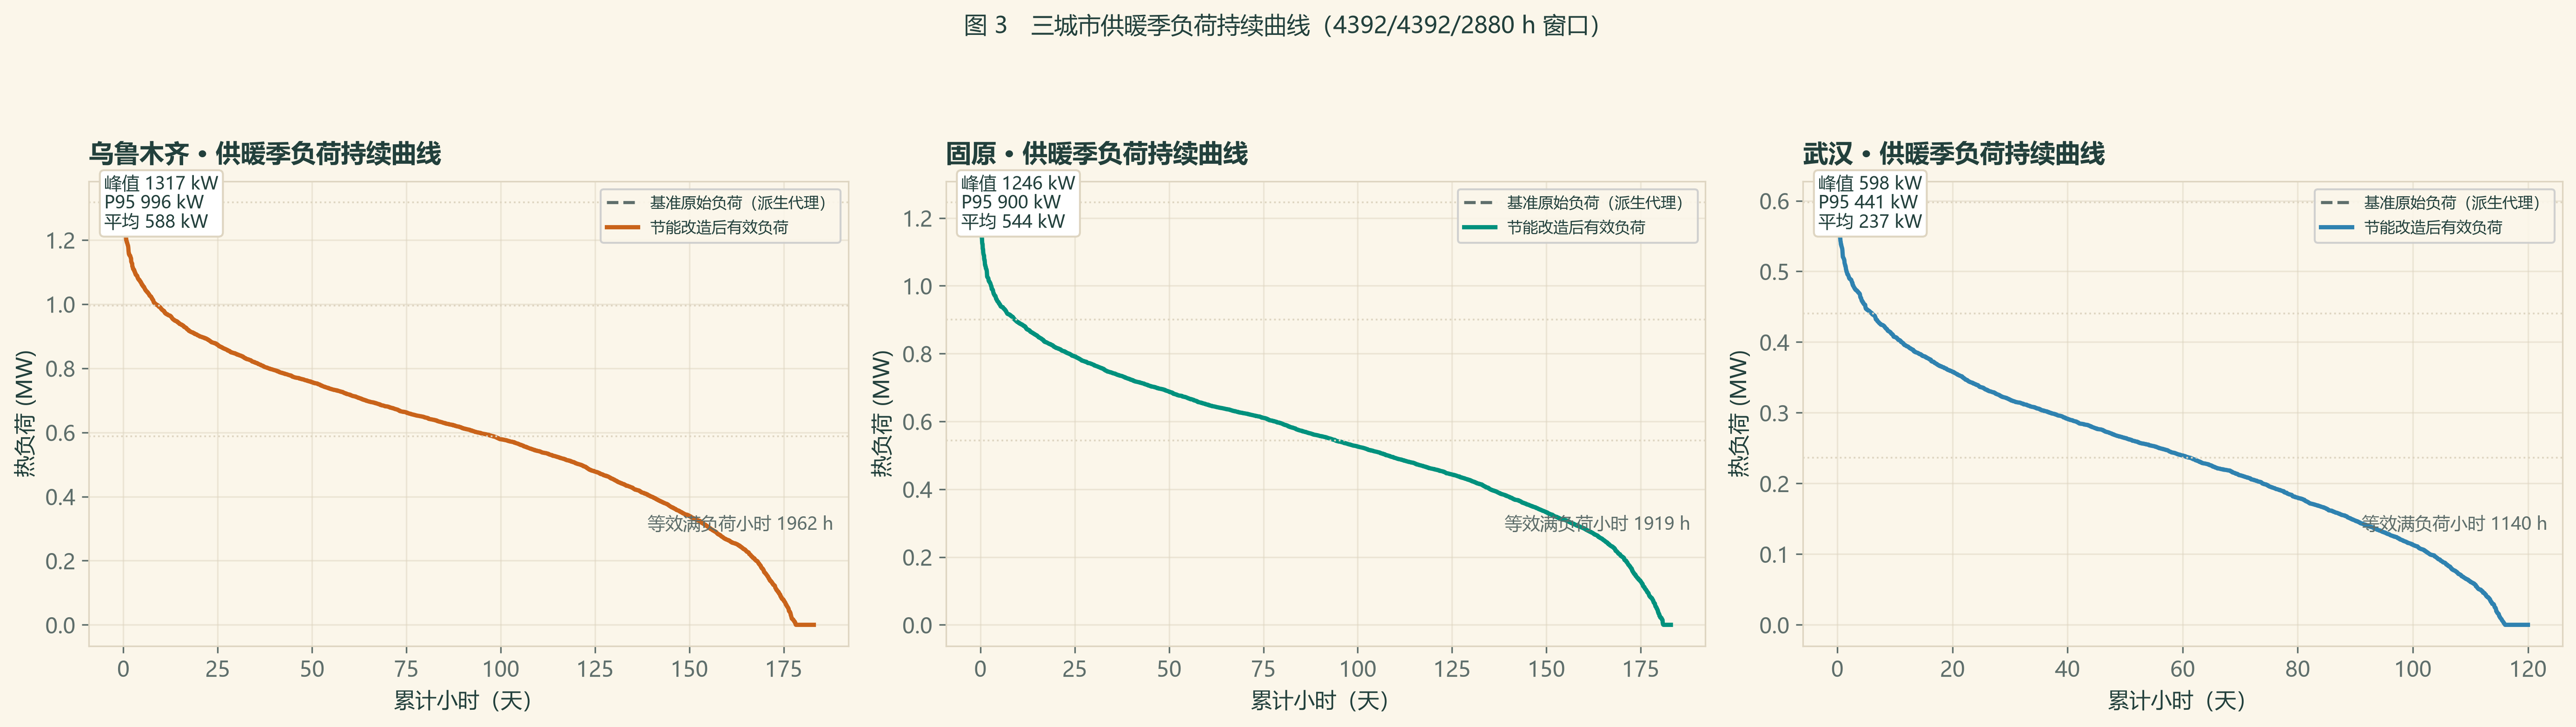
\includegraphics[width=0.98\textwidth,height=0.44\textheight,keepaspectratio,trim=0 0 0 100,clip]{media/code-results/fig03_load_duration_curve.png}
\caption{三城市供暖季负荷持续曲线}
\label{fig:code-load-duration}
\end{figure}

\subsection{模型结构}

模型以建筑逐时负荷为入口，将规划期内的热源建设、设备退役、管网改造、储热配置和配电增容，与供暖季内的热源出力、管网输配、储热充放和建筑热状态统一描述。三个算例均设置3个模型节点，其中2个为聚合需求节点；乌鲁木齐、固原和武汉分别配置7、6、7类热源以及3、2、1条聚合管段。城市层确定资产配置与建设时序，区域层描述热源、管段、换热站和储热之间的能量传输，用户层以聚合节点承载典型建筑负荷与可调节热状态。城市、区域和用户表示决策尺度，不与模型节点逐一对应；算例节点不等同于完整城市地理网络。

公用模型内核包含负荷预测、热源转换、节点平衡、管网输配、储热递推、电力平衡和可靠性约束；场景适配模块根据城市的既有资产、资源条件、网络结构和服务需求加载专用约束。整体关系如图\ref{fig:model-cn-overall}所示。

$n,e,b,k,s$分别表示节点、管段、建筑、热源和储热设备，$g,y,t$为温位、阶段和小时。单阶段算例固定$y$。乌鲁木齐联合求解投资与运行，固原、武汉锚定投资后逐时校核。\textbf{温位、输配、建筑柔性与储热共同约束规划配置。}

\begin{figure}[H]
\centering
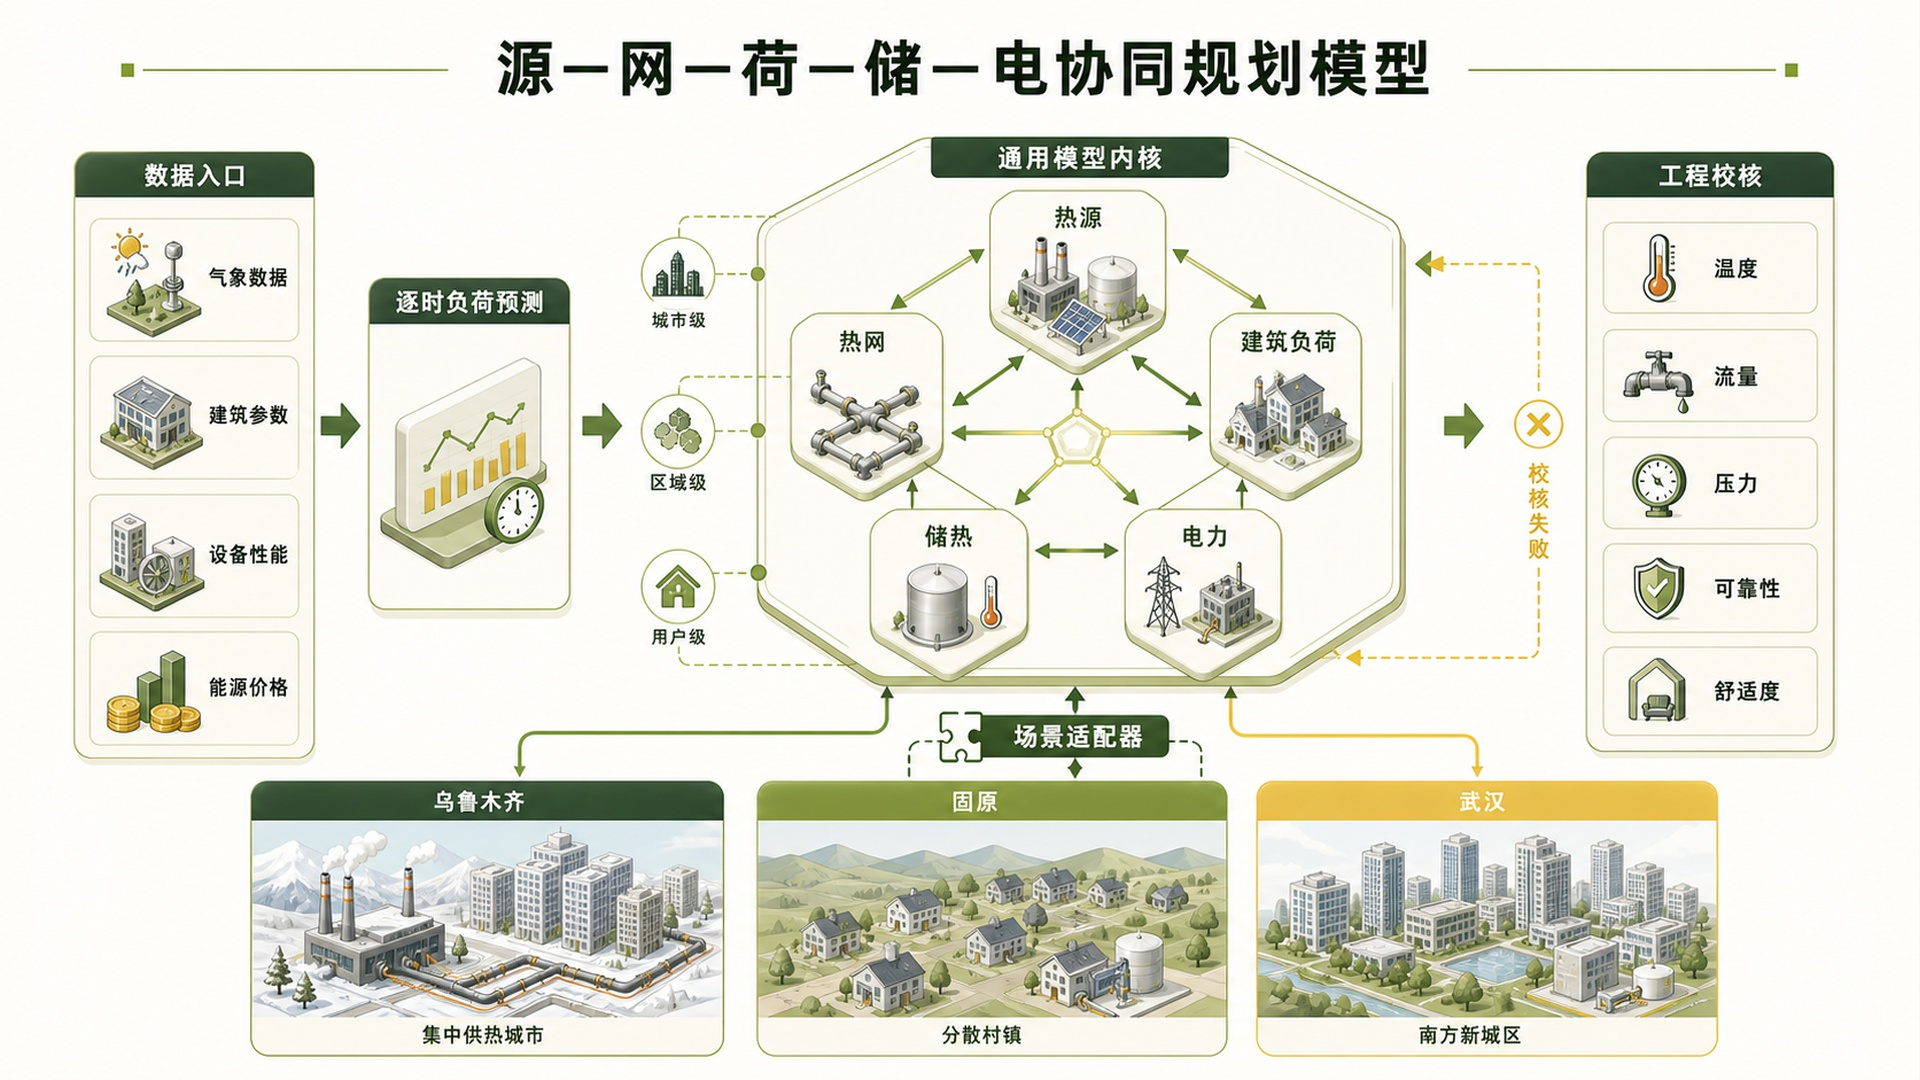
\includegraphics[width=0.76\textwidth,height=0.38\textheight,keepaspectratio]{media/model-cn/01_总体模型框架.jpg}
\caption{协同规划模型框架}
\label{fig:model-cn-overall}
\end{figure}

规划、运行和工程校核采用分层衔接方式。规划层确定建设与容量方案，运行层完成逐时调度；本次数值校核包括热平衡、容量、储热状态、配电边界和失供量检查，工程复核包括温位、关键管段和回水边界。原始算例以事后校核为主；新增有限模式反馈验证另列于表\ref{tab:minor-evidence}。计算流程如图\ref{fig:model-cn-loop}所示。

\begin{figure}[H]
\centering
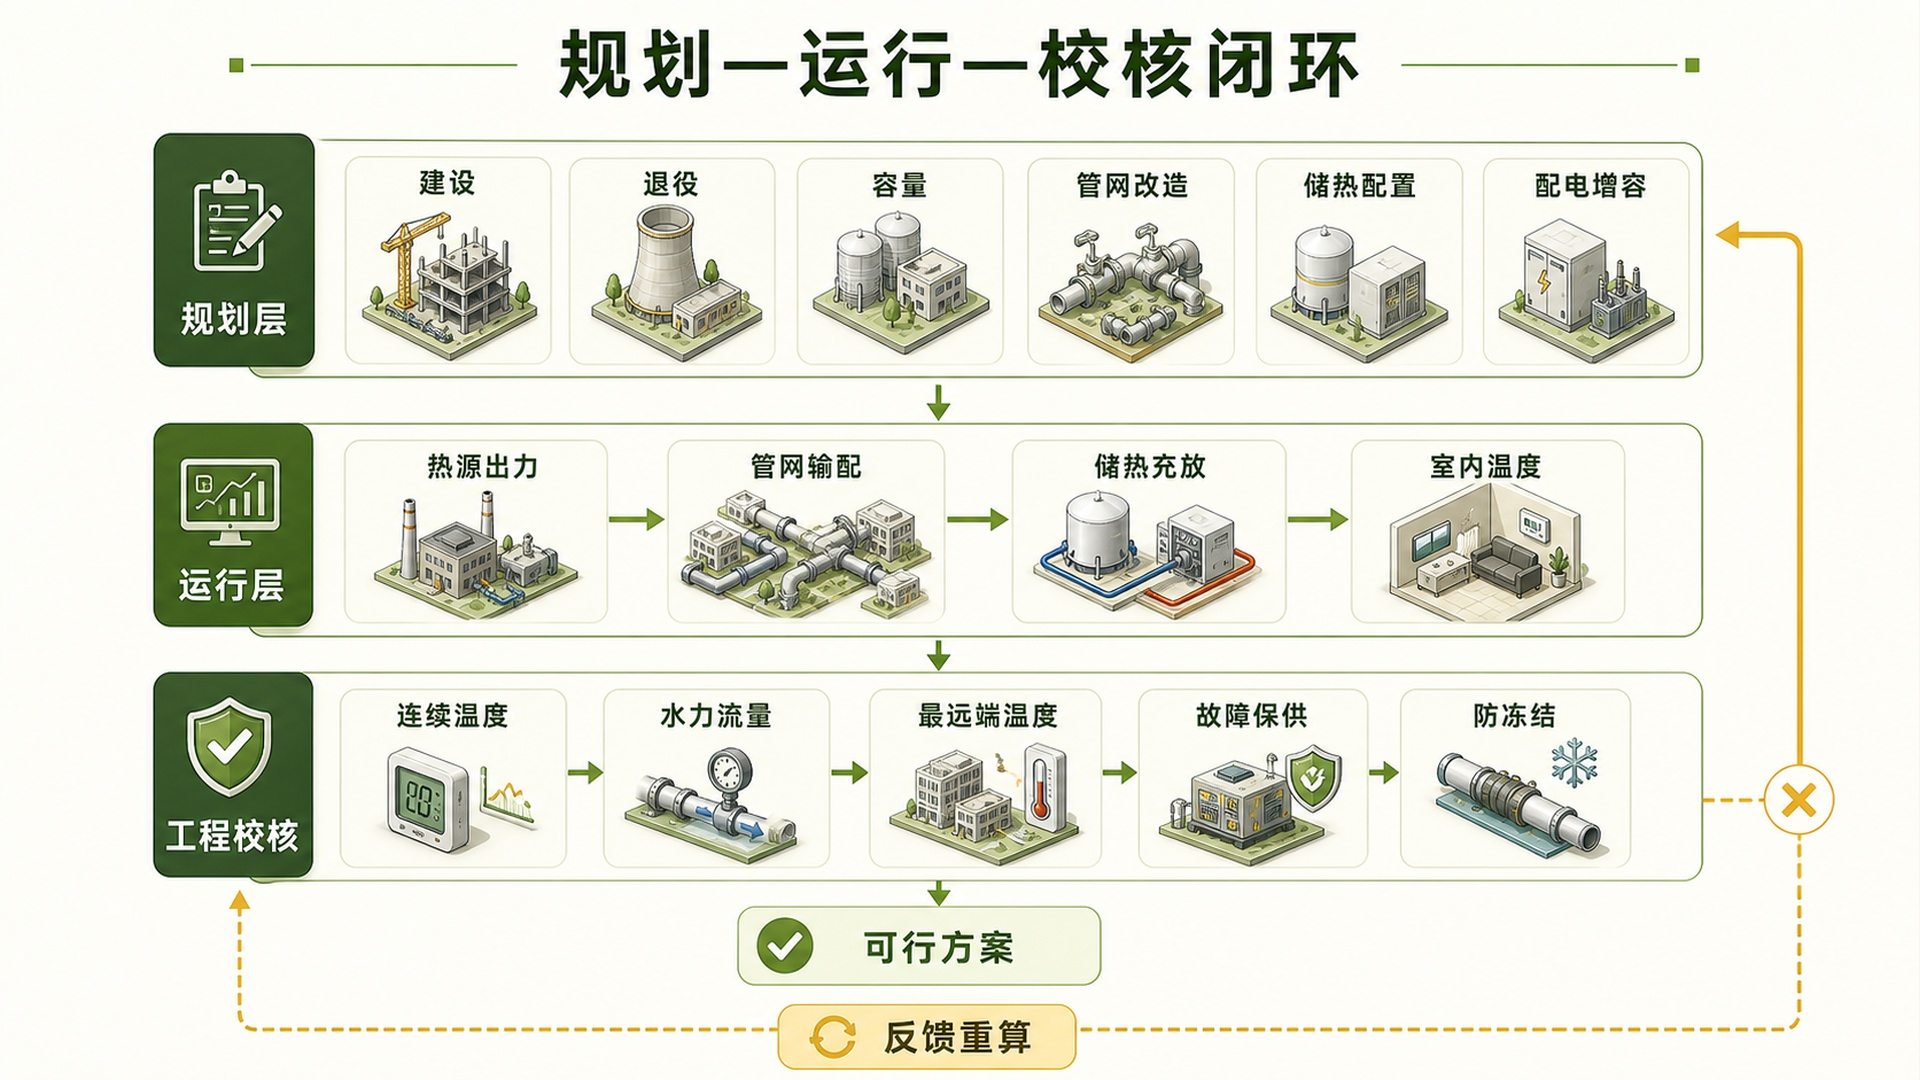
\includegraphics[width=0.76\textwidth,height=0.36\textheight,keepaspectratio]{media/model-cn/05_规划运行校核闭环.jpg}
\caption{规划与校核流程}
\label{fig:model-cn-loop}
\end{figure}

\subsection{建筑负荷}

\subsubsection{负荷分解}

建筑供热负荷由围护结构传热、渗透换气和机械新风热损失构成，同时扣除太阳辐射及人员、设备等内部得热：
\begin{equation}
Q_{b,t}^{\mathrm{load}}=Q_{b,t}^{\mathrm{trans}}+Q_{b,t}^{\mathrm{inf}}+Q_{b,t}^{\mathrm{vent}}-Q_{b,t}^{\mathrm{sol}}-Q_{b,t}^{\mathrm{int}}.
\label{eq:load-decomp}
\end{equation}
围护结构传热与渗透换气损失分别为
\begin{align}
Q_{b,t}^{\mathrm{trans}}&=U_bA_b\left(\theta_{b,t}^{a}-T_t^{\mathrm{out}}\right),\\
Q_{b,t}^{\mathrm{inf}}&=\frac{\rho_ac_an_b^{\mathrm{inf}}V_b}{3.6\times10^6}
\left(\theta_{b,t}^{a}-T_t^{\mathrm{out}}\right).
\end{align}
式中，$U_b$为综合传热系数，使用kW/(m$^2$\,$\cdot$\,K)；若原始值为W/(m$^2$\,$\cdot$\,K)，先除以1000。$A_b$为围护结构面积，$n_b^{\mathrm{inf}}$为换气次数（次/h），$V_b$为建筑体积；当$\rho_a$取kg/m$^3$、$c_a$取J/(kg$\cdot$K)时，除以$3600$完成小时换算，再除以$1000$得到kW。负荷分解关系见图\ref{fig:model-cn-load}。

基准负荷取非负值；建筑热工参数分别登记，调节后的供热量进入节点平衡。

\begin{figure}[H]
\centering
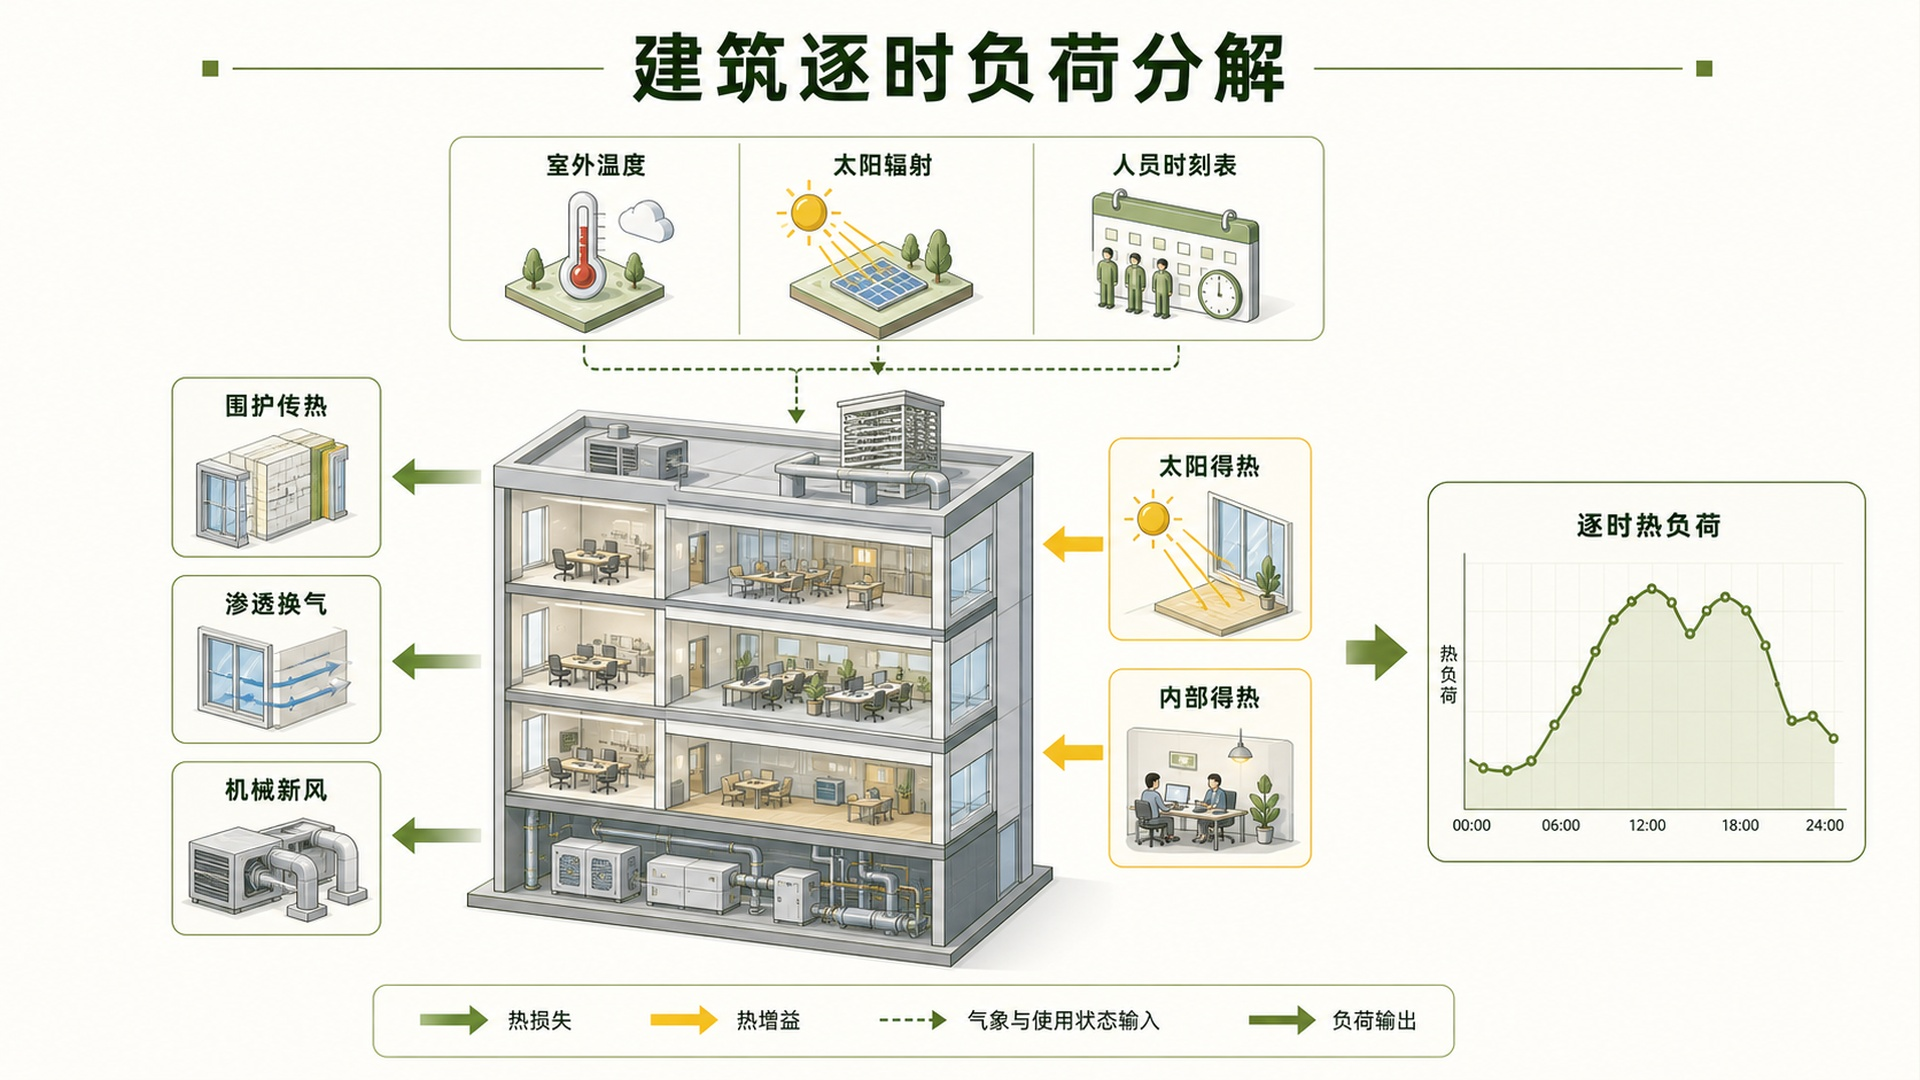
\includegraphics[width=0.76\textwidth,height=0.36\textheight,keepaspectratio]{media/model-cn/02_建筑逐时负荷分解.jpg}
\caption{建筑逐时负荷分解}
\label{fig:model-cn-load}
\end{figure}

\subsubsection{热惯性模型}

原始参数化算例采用单一等效热状态表示用户侧热惯性。令$E_{b,t}$为相对基准状态的蓄热量，$C_b$为聚合节点等效热容，$q_{b,t}^{+}$和$q_{b,t}^{-}$分别表示相对基准的负荷增加量和削减量，$\lambda_b$为每个时间步的衰减率，则
\begin{align}
E_{b,t}&=(1-\lambda_b)E_{b,t-1}+\left(q_{b,t}^{+}-q_{b,t}^{-}\right)\Delta t,\\
\Delta\theta_{b,t}&=\frac{E_{b,t}}{C_b},\qquad \Delta t=1~\mathrm h.
\end{align}
等效温度偏移受上下界约束，需求响应仅在允许窗口内转移负荷，并满足全窗口能量守恒。图\ref{fig:model-cn-2r2c}保留原有双状态概念示意；历史算例采用上述单一等效热状态。新增验证采用下述1R1C递推，分别记录模型版本。

令$D^0_{b,t}$为基准需求，聚合分支的调节量与节点需求通过下式连接：
\begin{align}
Q^{\mathrm h}_{b,t}&=D^0_{b,t}+q^+_{b,t}-q^-_{b,t},&
\underline{\Delta\theta}_b&\le E_{b,t}/C_b\le\overline{\Delta\theta}_b,\\
D_{n,g,t}&=\sum_{b\in\mathcal B_{n,g}}Q^{\mathrm h}_{b,t}+D^{\mathrm{DHW}}_{n,g,t}.
\label{eq:r8m-load-interface}
\end{align}
$\mathcal B_{n,g}$为该节点温位的建筑集合，生活热水按配置计入，建筑供热不重复归集。

\begin{figure}[H]
\centering
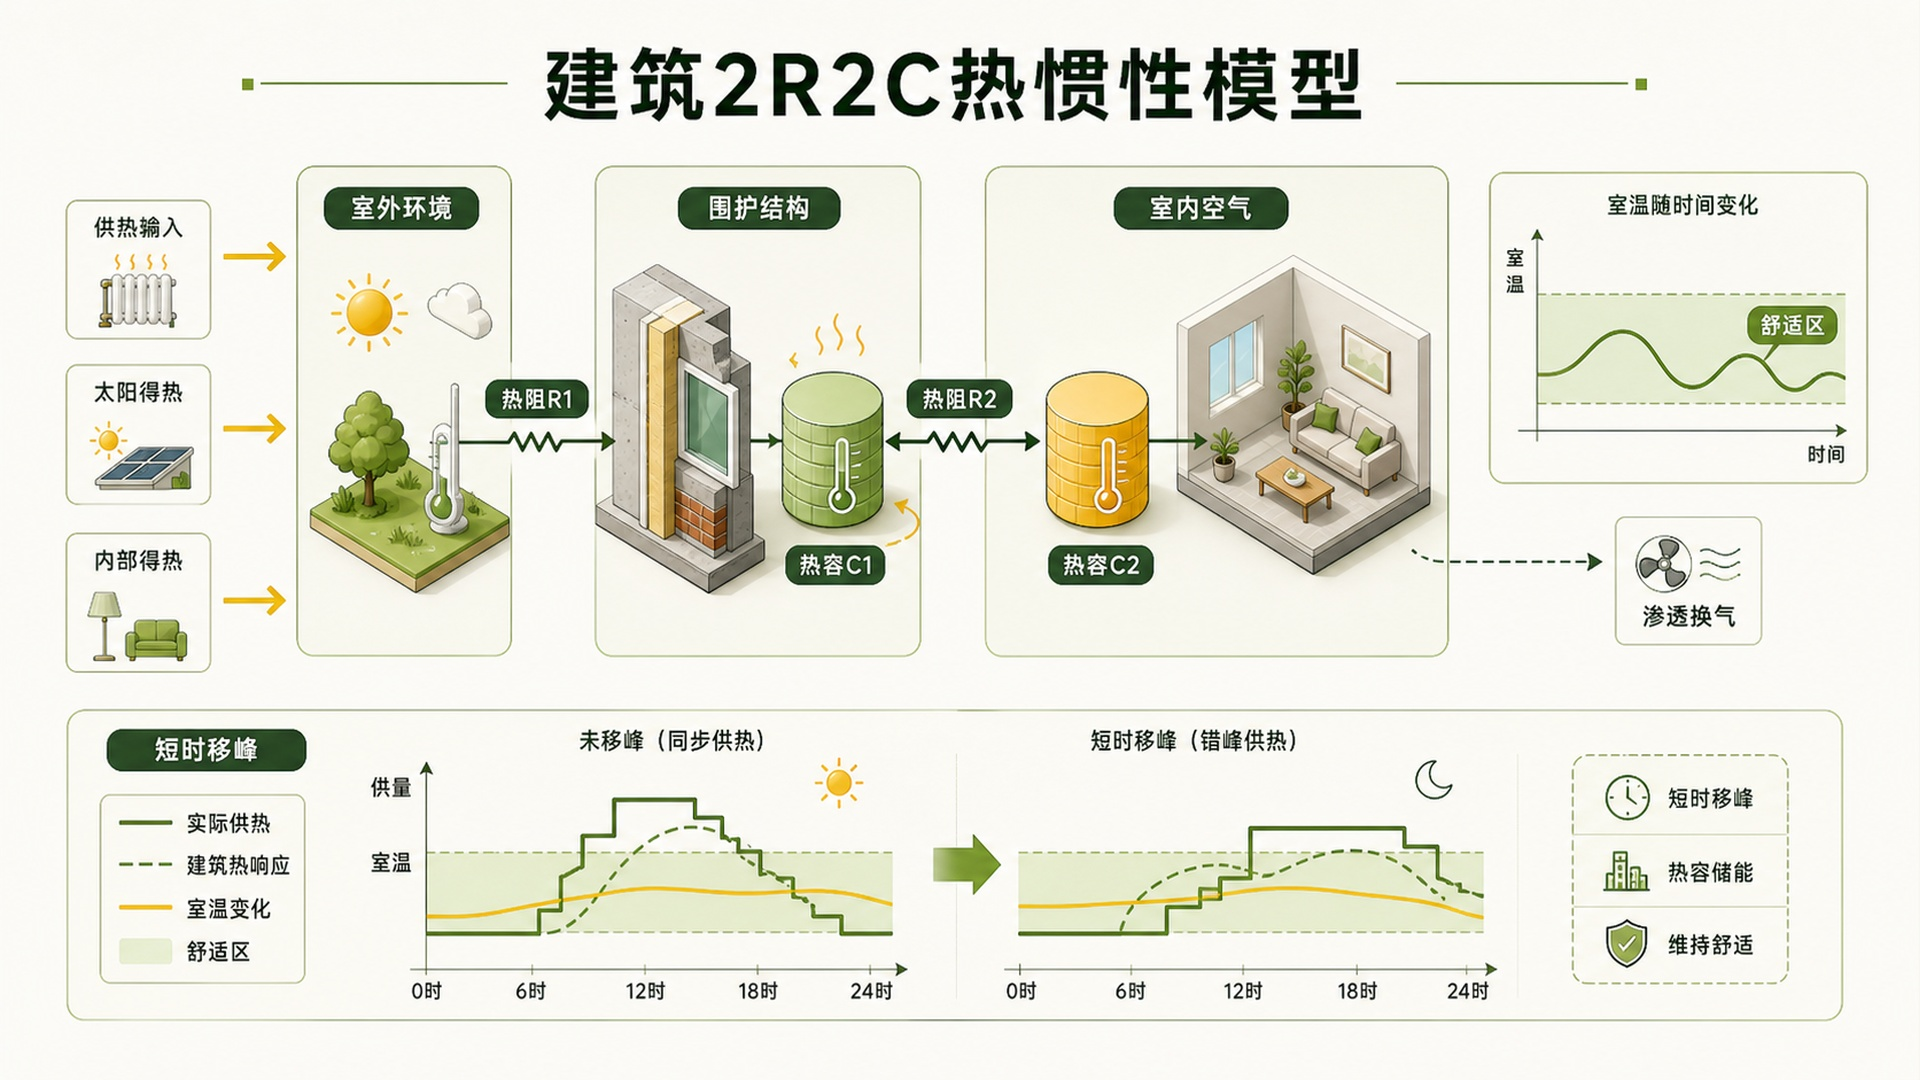
\includegraphics[width=0.76\textwidth,height=0.36\textheight,keepaspectratio]{media/model-cn/03_建筑2R2C热惯性.jpg}
\caption{建筑热惯性概念结构（原框架示意）}
\label{fig:model-cn-2r2c}
\end{figure}


\noindent\textbf{热状态实现的补充。}新增逐楼验证采用1R1C模型\supcite{28}。令$H_b$为围护与换气总热损失系数（kW/K），$C_b$为有效热容（kWh/K），$G_{b,t}$为太阳和内部得热，则在每小时输入不变时，精确积分得到
\begin{equation*}
\begin{aligned}
a_b&=\exp(-H_b\Delta t/C_b),\qquad \beta_b=(1-a_b)/H_b,\\
\theta_{b,t}&=a_b\theta_{b,t-1}+(1-a_b)T_t^{\mathrm{out}}
+\beta_b(Q_{b,t}^{\mathrm h}-Q_{b,t}^{\mathrm c}+G_{b,t}).
\end{aligned}
\end{equation*}
室温满足逐时舒适边界，供热与供冷受设备能力及所选互斥约束限制。初末室温固定，避免通过消耗末态蓄热降低费用；供热量进入节点平衡，电耗汇入公共配电。该分支保留预热造成的额外散热，相关实验与原聚合需求响应结果分开报告。

$\theta_{b,t}$为小时末室温，满足$\underline\theta_{b,t}\le\theta_{b,t}\le\overline\theta_{b,t}$；两类热状态按算例选用，分别得到建筑供热量后，再按节点与温位求和归集。

\subsection{协同约束}

\subsubsection{容量与出力}

设备在规划阶段的可用容量由既有、新建和退役容量共同决定：
\begin{equation}
K_{k,y}=K_k^{\mathrm{exist}}+\sum_{\tau\leq y}K_{k,\tau}^{\mathrm{new}}-\sum_{\tau\leq y}K_{k,\tau}^{\mathrm{ret}}.
\end{equation}
热源逐时出力满足
\begin{equation}
\underline Q_k u_{k,t}\leq Q_{k,t}\leq \overline Q_k u_{k,t},
\qquad Q_{k,t}\leq a_{k,t}K_{k,y},
\end{equation}
其中$u_{k,t}$为启停状态，$a_{k,t}$为可用率。锅炉和热泵的能量转换关系分别为
\begin{equation}
Q_{k,t}^{\mathrm{boiler}}=\eta_k^{\mathrm{boiler}}F_{k,t}^{\mathrm{fuel}},
\qquad Q_{k,t}^{\mathrm{HP}}=COP_{k,t}P_{k,t}^{\mathrm{HP}}.
\end{equation}

燃料输入按低位热值折为kW；热泵取热量为$Q^{\mathrm{HP}}-P^{\mathrm{HP}}$。热电联产满足$\alpha_k^{\min}Q_{k,t}^{\mathrm{CHP}}\le P_{k,t}^{\mathrm{CHP}}\le\alpha_k^{\max}Q_{k,t}^{\mathrm{CHP}}$，售电单列计价；启停与爬坡按配置加载。

\subsubsection{热量平衡}

对节点$n$、温位$g$和时刻$t$，热源输入、上游来热和储热放热应等于用户负荷、储热充热和下游送热：
\begin{multline}
\sum_k Q_{k,n,g,t}+\sum_{a\in\delta^-(n)}\eta_aF_{a,g,t}+\sum_sQ_{s,n,g,t}^{\mathrm{dis}}\\
=D_{n,g,t}+\sum_sQ_{s,n,g,t}^{\mathrm{ch}}+\sum_{a\in\delta^+(n)}F_{a,g,t}.
\label{eq:node-heat-balance}
\end{multline}
该约束按节点、温位和时段分别建立，避免使用全系统总量平衡掩盖局部输配不足。源、网、荷、储、电之间的关系见图\ref{fig:model-cn-unified}。

各温位出力之和为热源总出力。$a$为有向连接，其$F_a$对应物理管段$e$的$F_e^+$或$F_e^-$。\textbf{各环节在同一小时闭合。}

\begin{figure}[H]
\centering
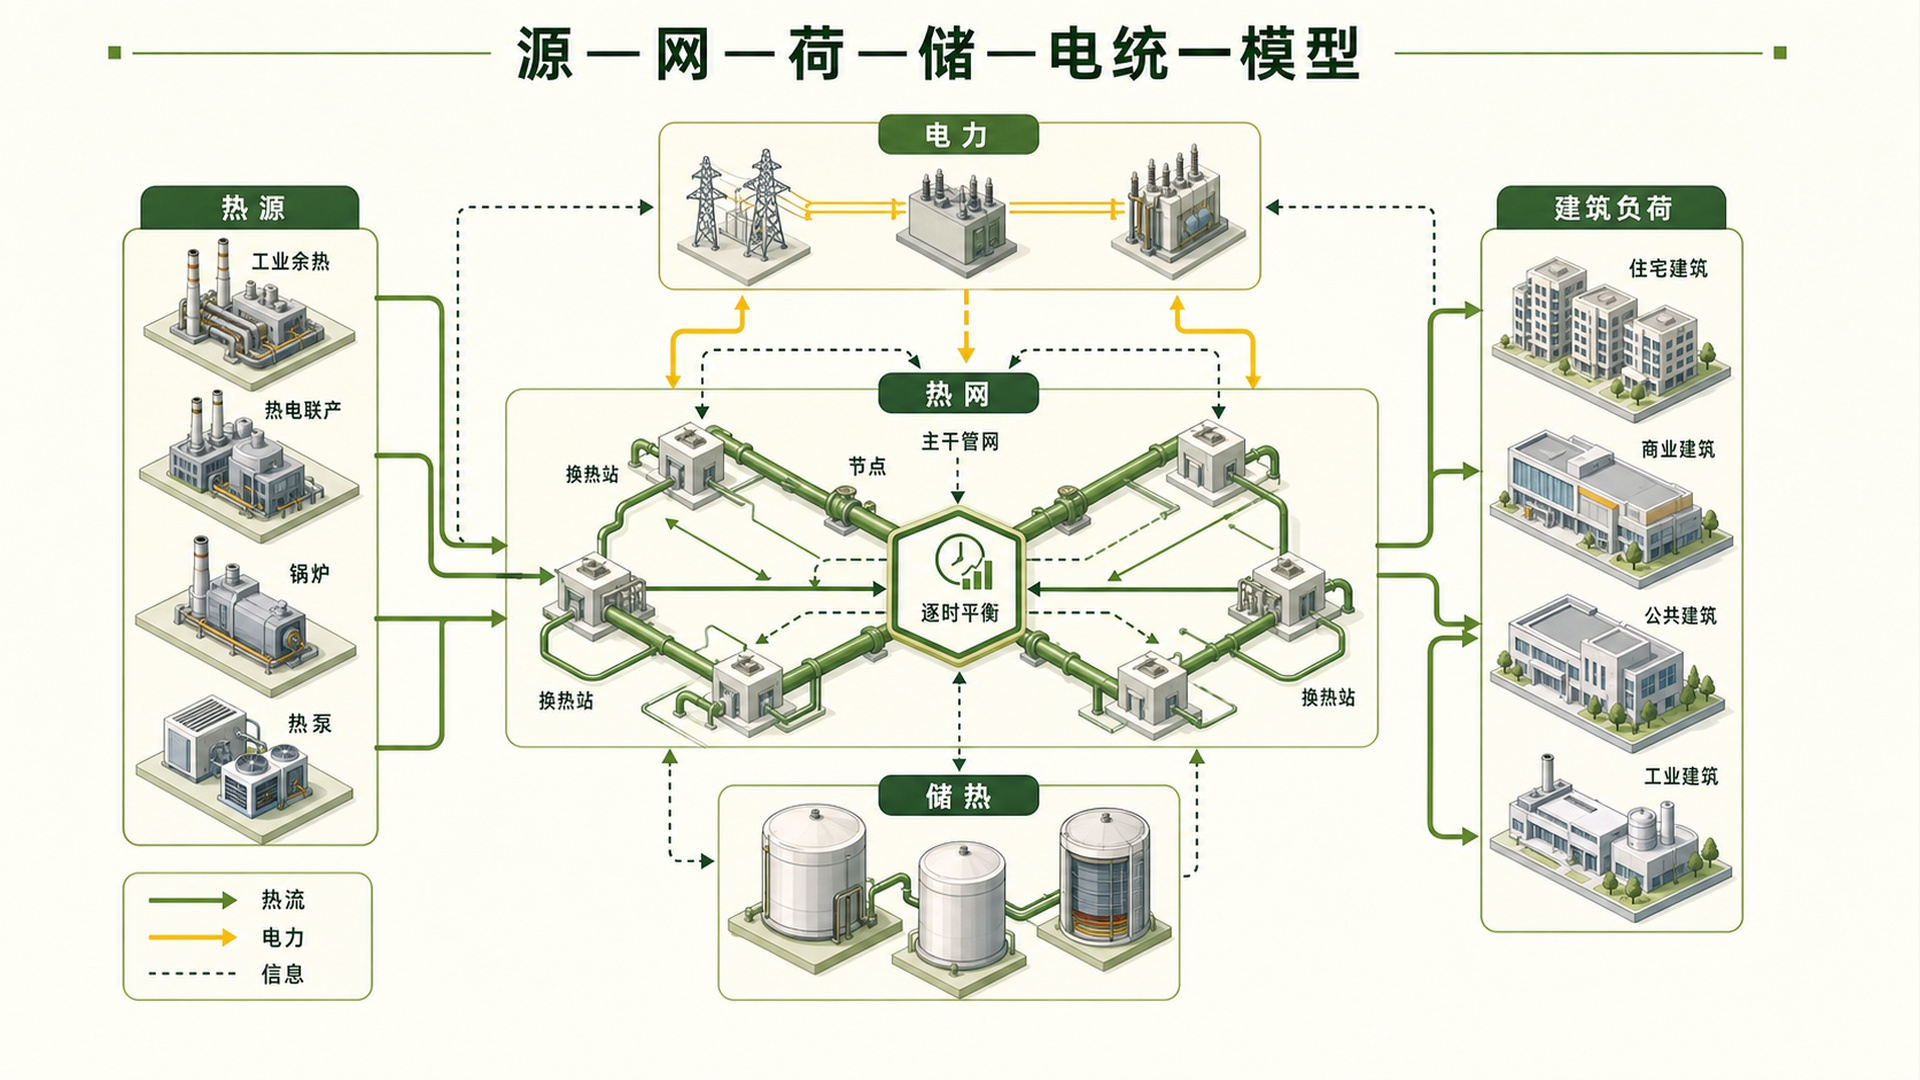
\includegraphics[width=0.76\textwidth,height=0.37\textheight,keepaspectratio]{media/model-cn/04_源网荷储电统一模型.jpg}
\caption{多能流协同关系}
\label{fig:model-cn-unified}
\end{figure}

\subsubsection{温位与管网}

直接供热路径启用时，热源最低供水温度应满足用户温位和换热端差要求：
\begin{equation}
T_k^{\mathrm{src,min}}\geq T_g^{\mathrm{sup}}+\Delta T^{\mathrm{hx}}.
\end{equation}
主模型采用固定温差将热流与质量流量关联：
\begin{equation}
F_{e,g,t}=c_p\Delta T_g\dot m_{e,g,t},
\qquad \sum_g(F^+_{e,g,t}+F^-_{e,g,t})\leq F_e^{\mathrm{exist}}+\sum_d\overline F_{e,d}z_{e,d}.
\end{equation}
温位不匹配的热源不得直接承担高温负荷，需要通过热泵等设备提升温度。梯级利用关系见图\ref{fig:model-cn-grade}。

两方向热流互斥，温级共享管段容量，$\sum_dz_{e,d}\le1$；$c_p$与流量分别采用kJ/(kg$\cdot$K)和kg/s。

\begin{figure}[H]
\centering
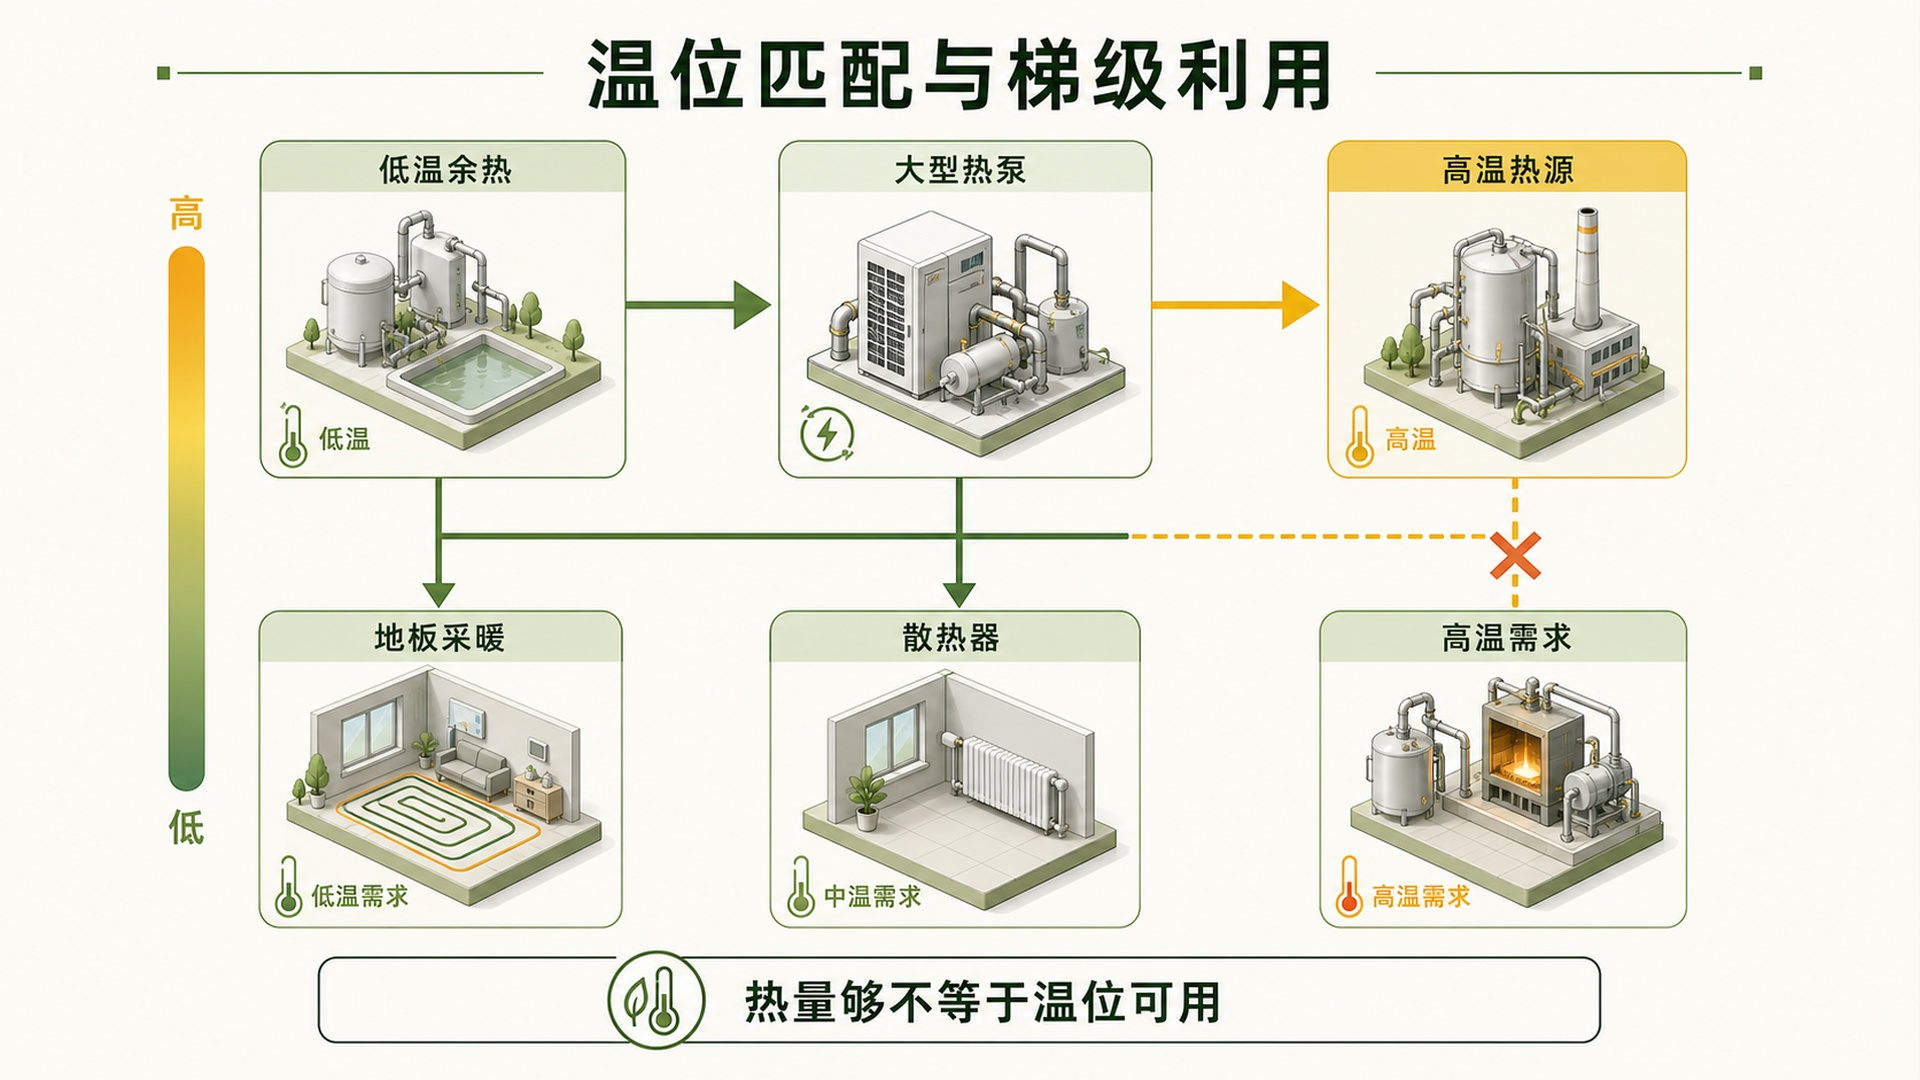
\includegraphics[width=0.76\textwidth,height=0.35\textheight,keepaspectratio]{media/model-cn/06_温位匹配与梯级利用.jpg}
\caption{温位匹配与梯级利用}
\label{fig:model-cn-grade}
\end{figure}

\subsubsection{储热与电力}

储热状态按时段递推：
\begin{equation}
E_{s,t}=(1-\mu_s)E_{s,t-1}+\eta_s^{\mathrm{ch}}Q_{s,t}^{\mathrm{ch}}\Delta t
-\frac{Q_{s,t}^{\mathrm{dis}}\Delta t}{\eta_s^{\mathrm{dis}}}.
\label{eq:storage-state}
\end{equation}

储热容量、充放功率及严格互斥模式的边界为
\begin{align}
0\le E_{s,t}&\le\overline E_s,&
0\le Q^{\mathrm{ch}}_{s,t}&\le\overline Q_s^{\mathrm{ch}},&
0\le Q^{\mathrm{dis}}_{s,t}&\le\overline Q_s^{\mathrm{dis}},\\
Q^{\mathrm{ch}}_{s,t}&\le M_s^{\mathrm{ch}}v_{s,t},&
Q^{\mathrm{dis}}_{s,t}&\le M_s^{\mathrm{dis}}(1-v_{s,t}),&v_{s,t}&\in\{0,1\}.
\end{align}
$\overline E_s$包含既有与新增容量，功率界随配置确定；$M$为候选静态上界。初末边界二选一：
\begin{equation}
\begin{cases}
E_{s,0}=\alpha_s^0\overline E_s,\quad E_{s,T}\ge\alpha_s^{\mathrm{end}}\overline E_s,&\text{固定边界},\\
E_{s,0}=E_{s,T},&\text{循环边界}.
\end{cases}
\end{equation}
能量与功率分别限制储热量和小时调节能力；跨季节应用另需连续覆盖充热季。
热泵、电锅炉、循环泵和储电设备共同进入电力平衡；原聚合算例按系统服务设备汇总：
\begin{multline}
P_t^{\mathrm{imp}}+P_t^{\mathrm{loc}}+P_t^{\mathrm{bat,dis}}\\
=P_t^{\mathrm{base}}+P_t^{\mathrm{HP}}+P_t^{\mathrm{EB}}
+P_t^{\mathrm{pump}}+P_t^{\mathrm{bat,ch}}+P_t^{\mathrm{exp}},\\
0\le P_t^{\mathrm{imp}}\le\overline P^{\mathrm{grid}}.
\end{multline}
储热充放时序与配电峰值的关系见图\ref{fig:model-cn-storage-grid}。

未启用项取零，供冷启用时计入电耗。$P^{\mathrm{loc}}$为公共平衡中的本地电源，独立售电的CHP不抵扣购电；逐楼模型另查楼栋限额。

\begin{figure}[H]
\centering
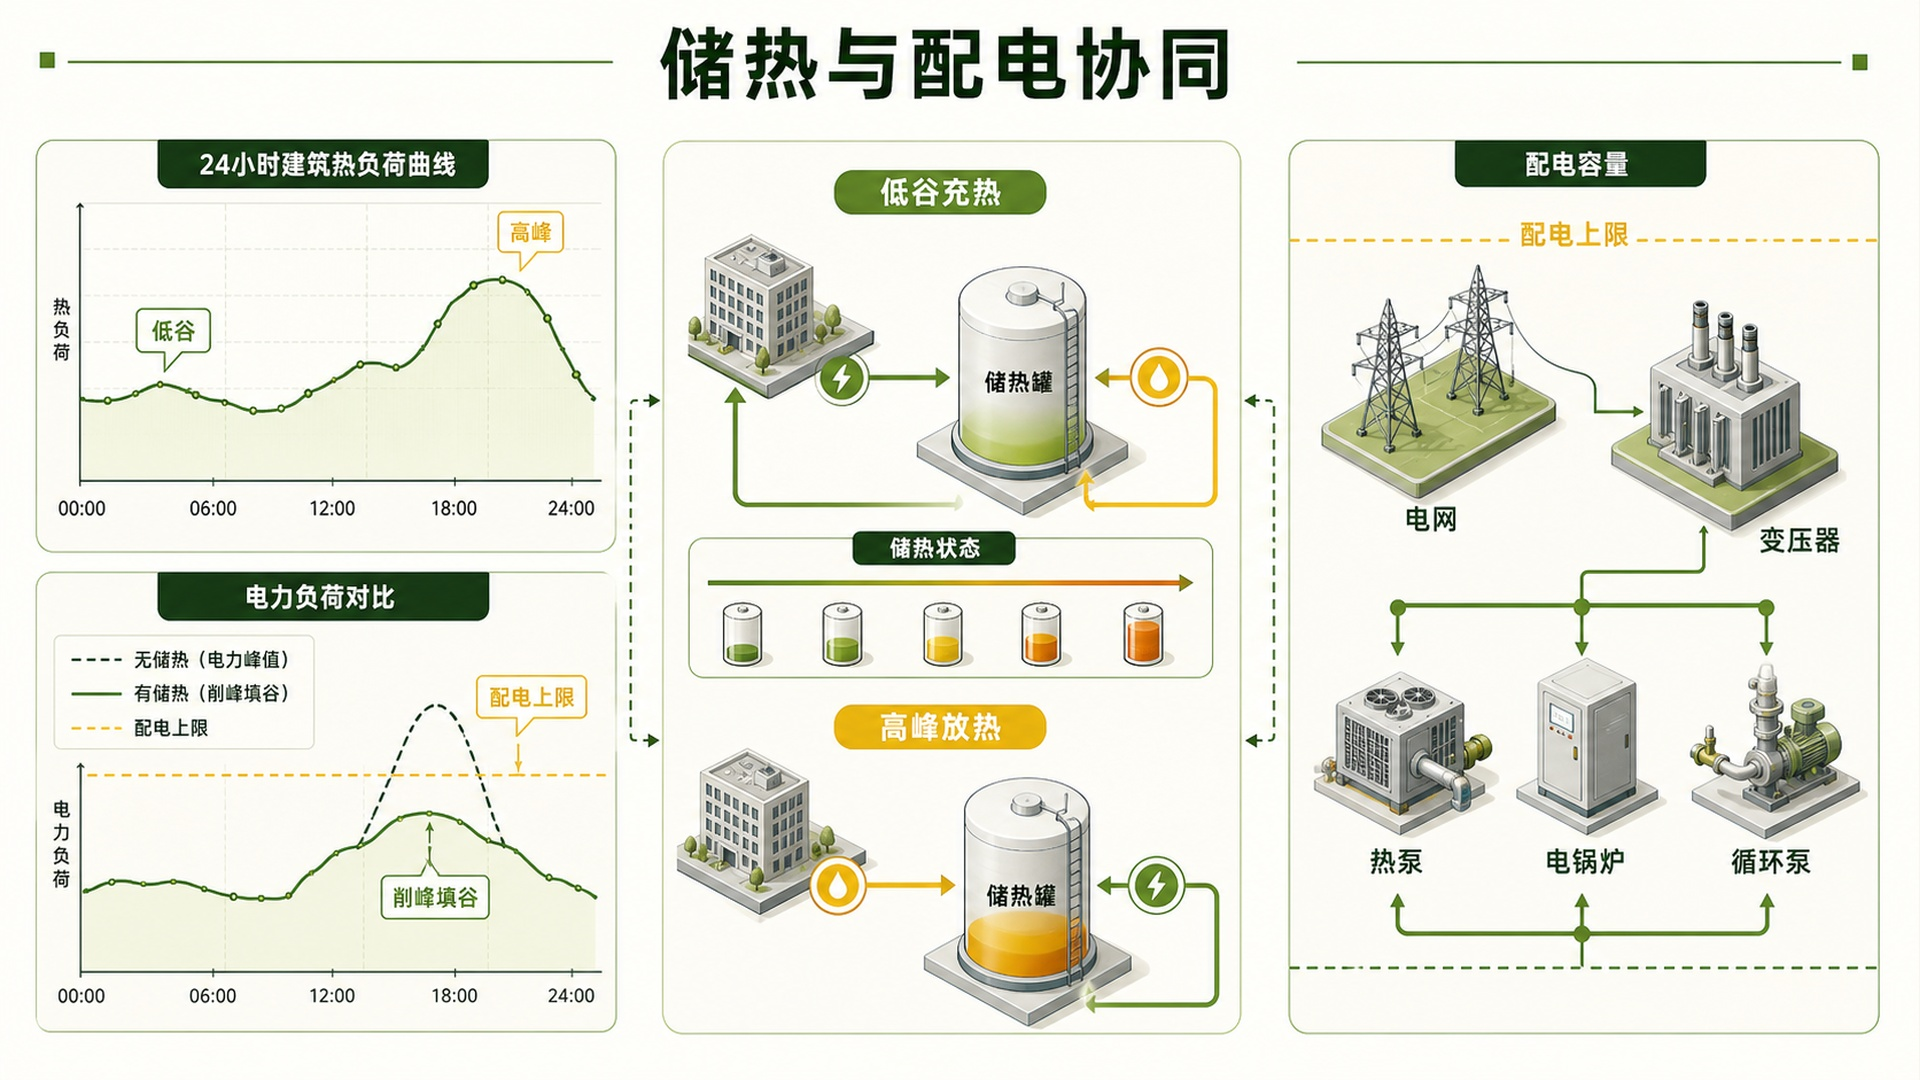
\includegraphics[width=0.76\textwidth,height=0.35\textheight,keepaspectratio]{media/model-cn/07_储热与配电协同.jpg}
\caption{储热与配电协同}
\label{fig:model-cn-storage-grid}
\end{figure}

\subsubsection{目标与可靠性}

模型以生命周期净成本$F^{\mathrm{cost}}$最小为基础目标，并通过$\varepsilon$约束控制碳排放。投资按5\%折现率和20年寿命折算为等年值，目标函数写为
\begin{align}
\min F^{\mathrm{cost}}={}&C^{\mathrm{ann,inv}}+C^{\mathrm{energy}}+C^{\mathrm{carbon}}
+C^{\mathrm{om}}+C^{\mathrm{pen}},\\
C^{\mathrm{ann,inv}}={}&\frac{r(1+r)^{20}}{(1+r)^{20}-1}C^{\mathrm{inv}},
\qquad r=5\%,\\
&F^{\mathrm{CO_2}}\leq\varepsilon_C.
\end{align}
其中$C^{\mathrm{energy}}$为能源费，$C^{\mathrm{carbon}}$为碳费，$C^{\mathrm{om}}$为运维费，$C^{\mathrm{pen}}$为火用失配与舒适偏差惩罚。实际现金成本仅包含发生的能源、运维和碳费用，不与惩罚项混合解释。

碳排放按登记的互不重复核算活动求和：
\begin{equation}
F^{\mathrm{CO_2}}=\sum_{j,t}\gamma_{j,t}A_{j,t}.
\end{equation}
$A$采用已积分活动量：供热与购电为$Q\Delta t$、$P\Delta t$（kWh），到货为本小时质量（kg；速率输入先乘$\Delta t$）。$\gamma$分别为kg~CO$_2$/kWh或kg~CO$_2$/kg。非电热源按供热因子、电驱设备按供电构成计排；启用的供冷与供应链另计，同一能源不重复登记。
失供率定义为
\begin{equation}
U^{\mathrm{un}}=\frac{\sum_tQ_t^{\mathrm{un}}}{\sum_tD_t}\leq\overline U.
\end{equation}
推荐方案取$\overline U=0$。严格平衡主模型中$Q_t^{\mathrm{un}}=0$。用户热状态、设备出力、温位、管网、储热和配电容量均作为硬约束，逐楼分支另执行室温边界，成本与碳排放在可行域内比较。约束关系见图\ref{fig:model-cn-objective}。

\begin{figure}[H]
\centering
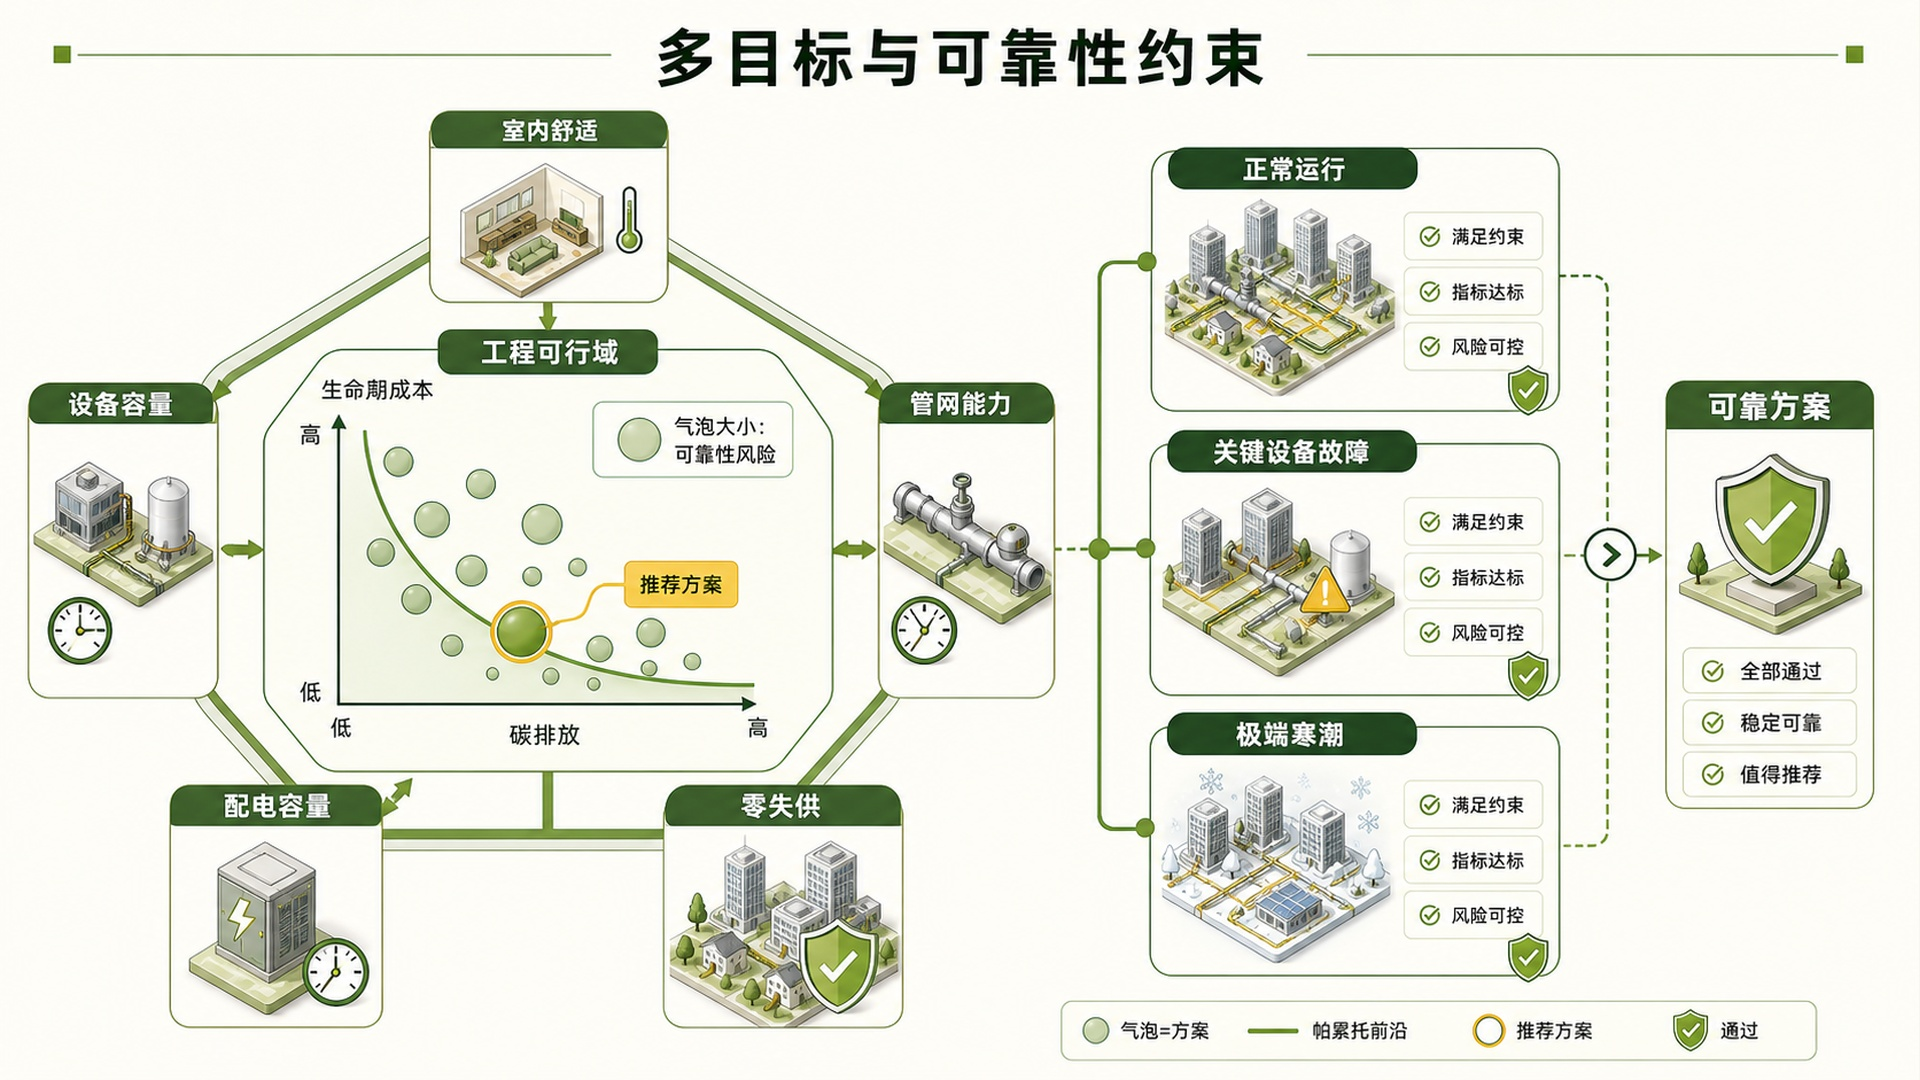
\includegraphics[width=0.76\textwidth,height=0.36\textheight,keepaspectratio]{media/model-cn/08_多目标与可靠性约束.jpg}
\caption{目标函数与可靠性约束}
\label{fig:model-cn-objective}
\end{figure}

\subsection{场景适配}

\subsubsection{乌鲁木齐场景}

乌鲁木齐以既有热电联产、骨干管网和换热站为基础，联合确定燃煤热源退役、工业余热接入、大型热泵、清洁调峰热源、储热及管网降温方案。退役容量必须由清洁热源、储热有效容量和备用容量共同补足：
\begin{equation}
K_{\mathrm{coal},y}^{\mathrm{ret}}\leq K_y^{\mathrm{clean,new}}+K_y^{\mathrm{storage,credit}}+K_y^{\mathrm{reserve}}.
\end{equation}
工业余热满足$0\leq Q_t^{\mathrm{waste}}\leq\overline Q_t^{\mathrm{waste}}$，温位不足时通过热泵升温。模型结构见图\ref{fig:model-cn-urumqi}。

储热有效容量采用满足峰值持续时间及状态边界的放热功率。\textbf{退役受可持续保供能力限制}，压力工况保持容量配置不变。

\begin{figure}[H]
\centering
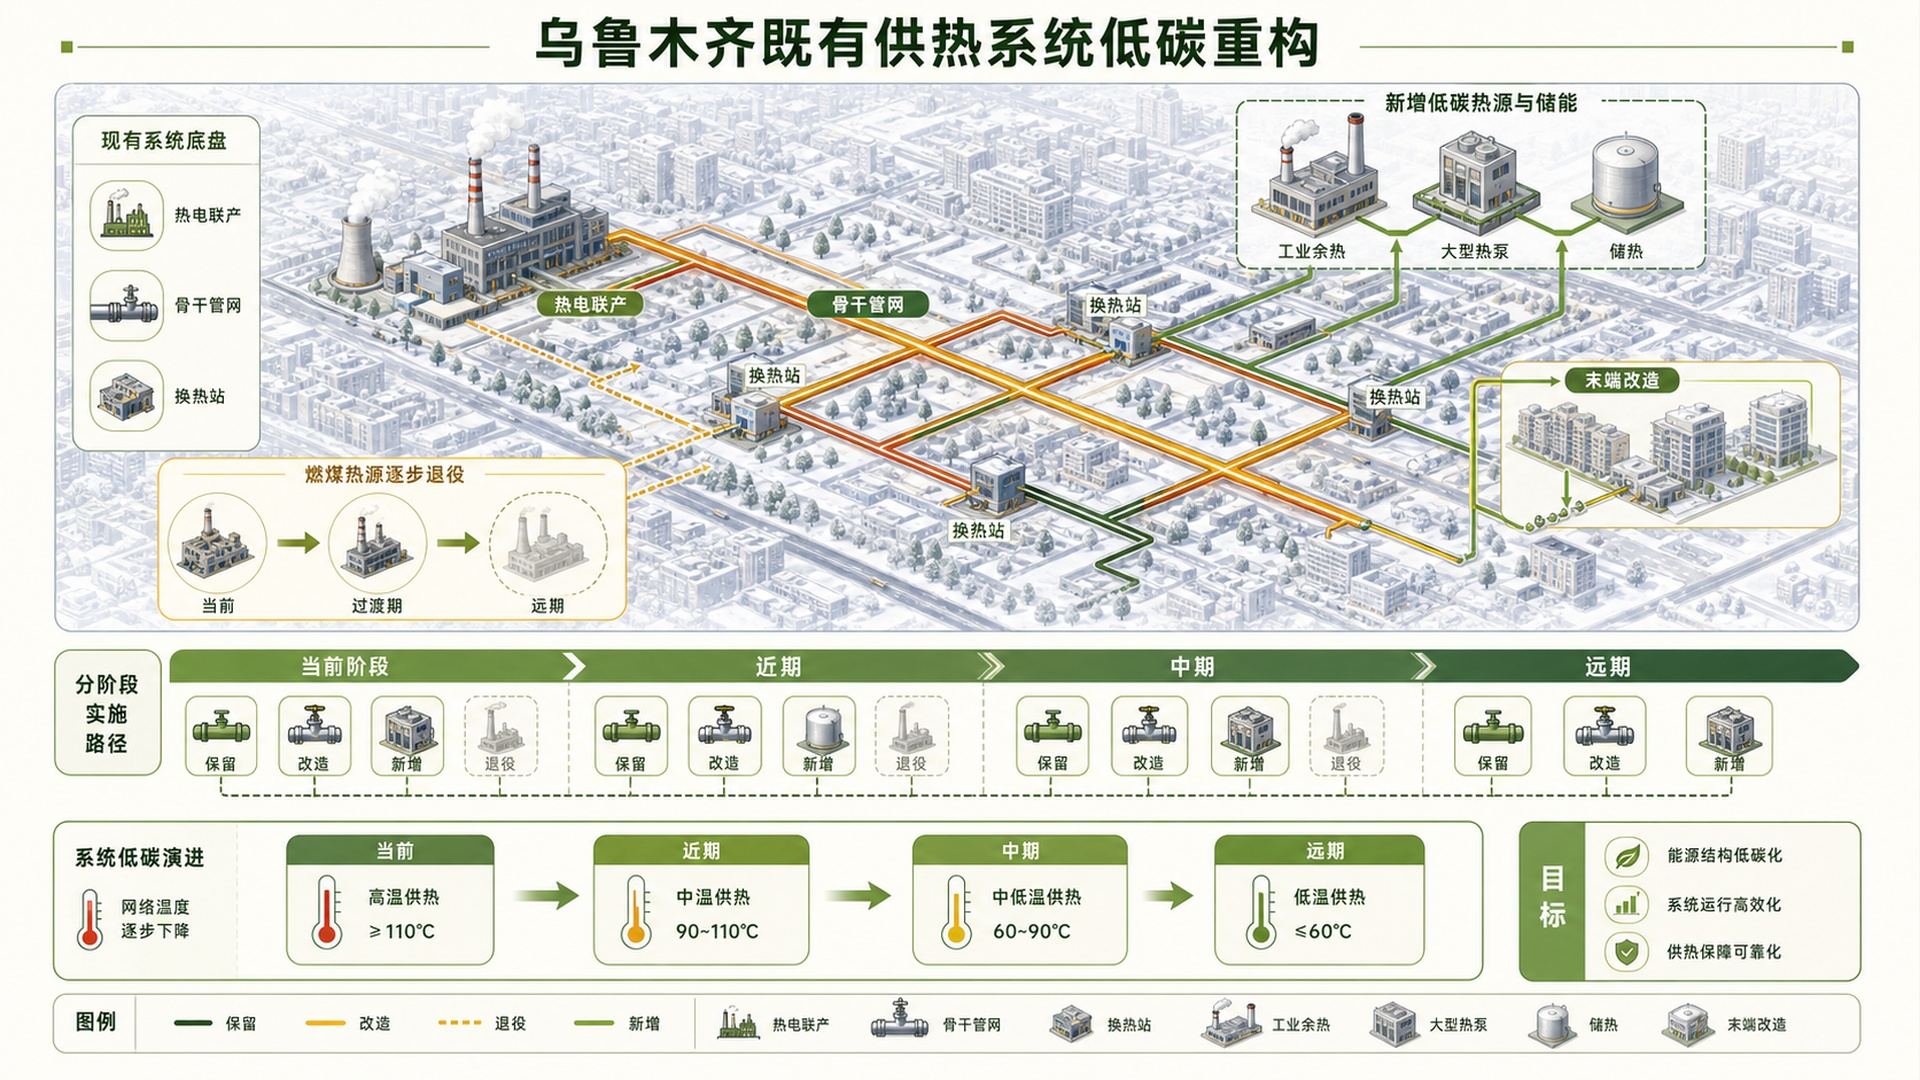
\includegraphics[width=0.77\textwidth,height=0.38\textheight,keepaspectratio]{media/model-cn/09_乌鲁木齐低碳重构.jpg}
\caption{乌鲁木齐低碳重构}
\label{fig:model-cn-urumqi}
\end{figure}

候选方案确定后，校核最远换热站供水温度、关键管段流量、回水温度、供回水温差、热源N-1、寒潮零失供以及管网降温与建筑末端改造的协调关系，见图\ref{fig:model-cn-urumqi-check}。详细约束列于附录1。

\begin{figure}[H]
\centering
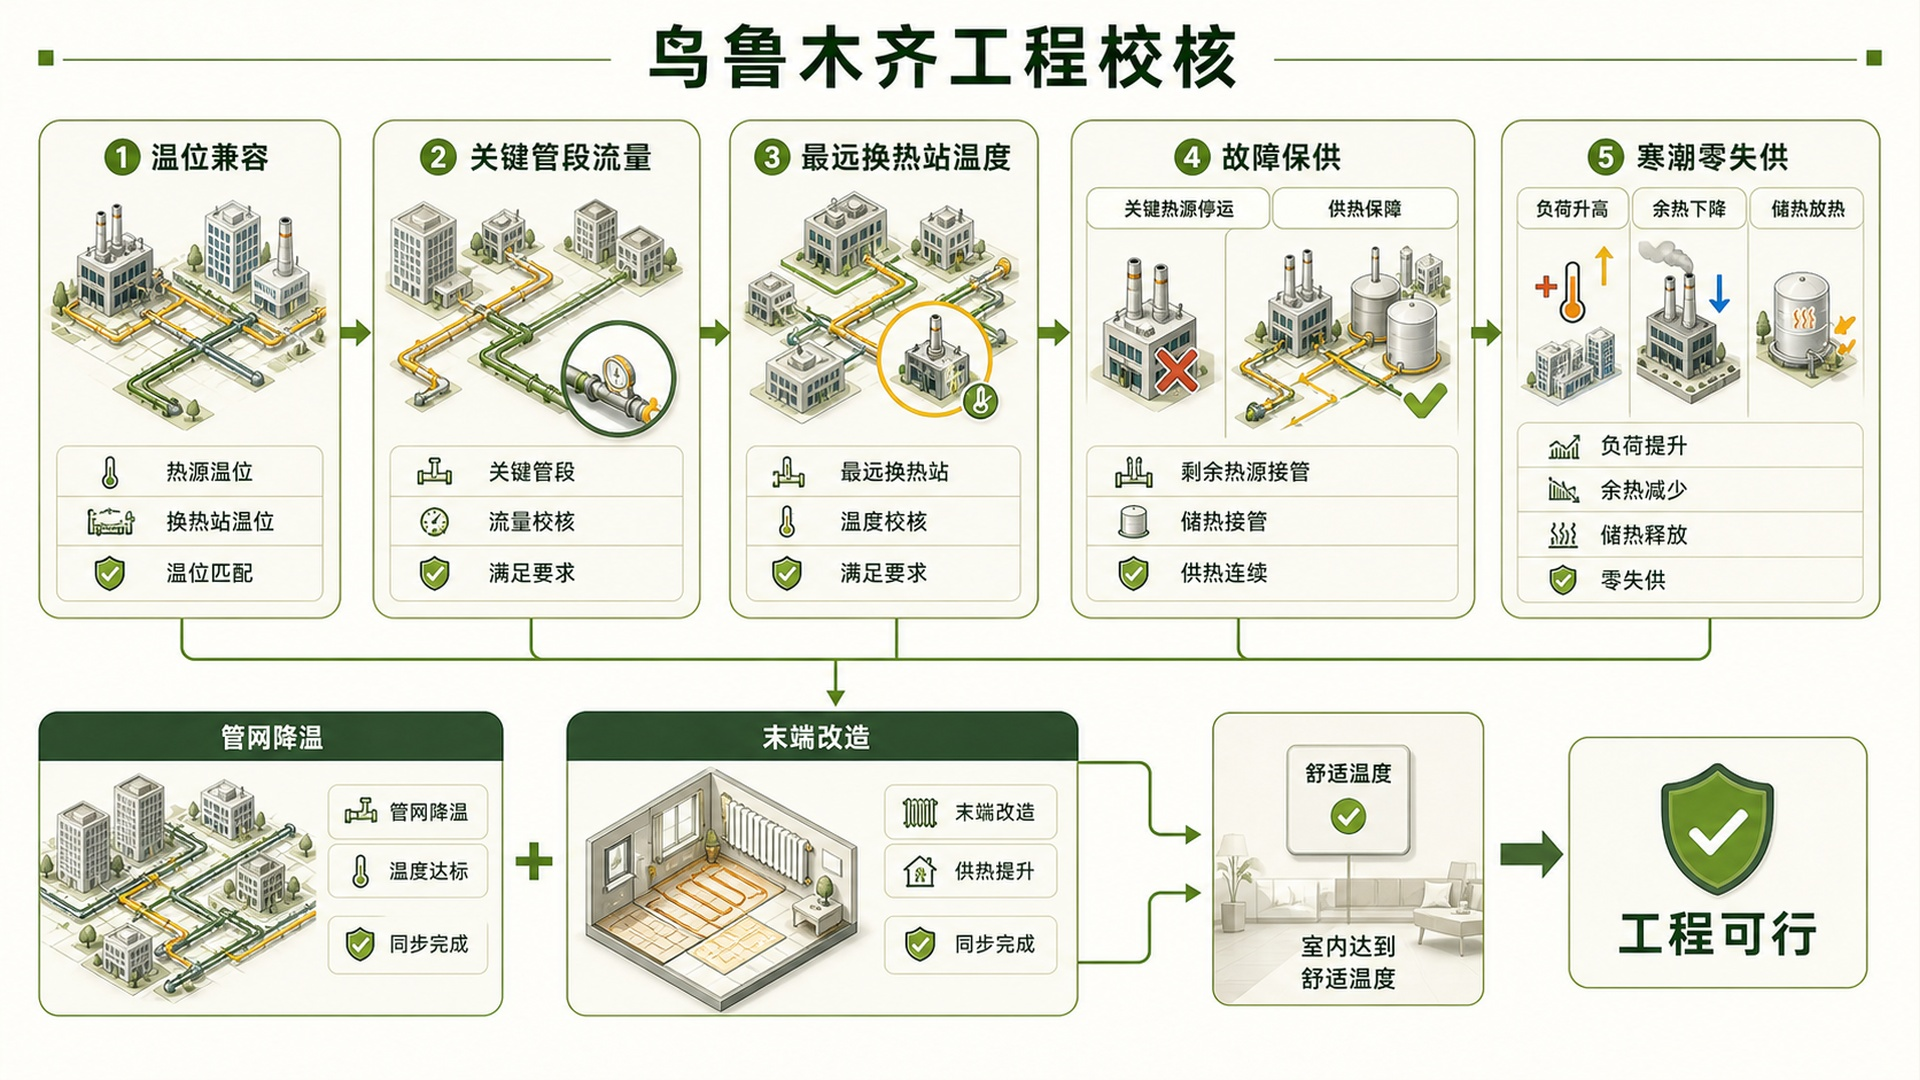
\includegraphics[width=0.76\textwidth,height=0.35\textheight,keepaspectratio]{media/model-cn/10_乌鲁木齐工程校核.jpg}
\caption{乌鲁木齐工程校核}
\label{fig:model-cn-urumqi-check}
\end{figure}

\subsubsection{固原场景}

固原以村镇、片区和区域微网为基本单元。原框架以如下选址和用户分配式定义空间组织接口；已报告算例在给定站点、用户归属及候选连接下求解容量与运行。扩展接口中，用户分配和服务半径满足
\begin{equation}
\sum_i x_{i,b}=1,\qquad x_{i,b}\leq z_i^{\mathrm{site}},\qquad
d_{i,b}x_{i,b}\leq\overline d_i,
\end{equation}
热源容量满足$\sum_bD_b^{\mathrm{peak}}x_{i,b}\leq K_i$。空间组织和技术配置见图\ref{fig:model-cn-guyuan}。

\begin{figure}[H]
\centering
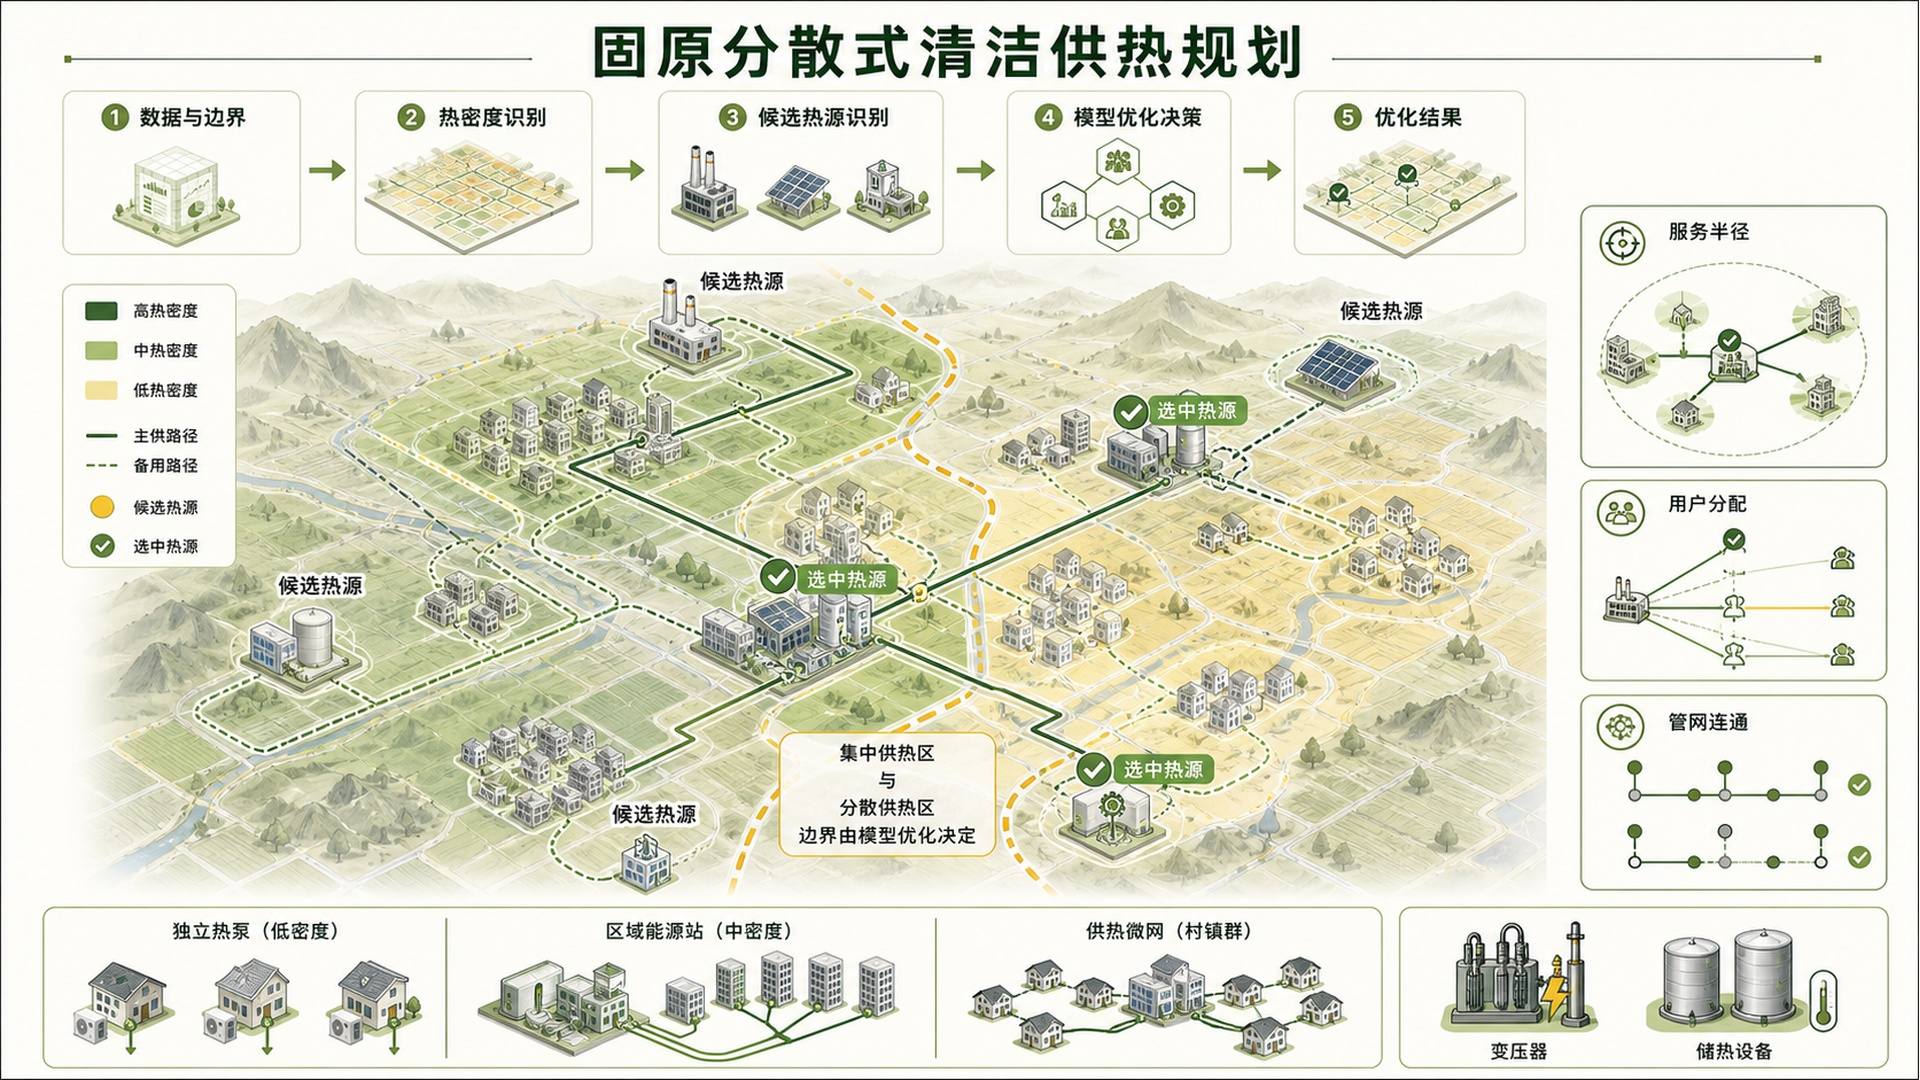
\includegraphics[width=0.77\textwidth,height=0.38\textheight,keepaspectratio]{media/model-cn/11_固原分散供热规划.jpg}
\caption{固原分散供热规划}
\label{fig:model-cn-guyuan}
\end{figure}

生物质燃料按到货、库存和消耗逐时递推，并在电网或单一热源故障下检查关键用户保供。燃料供应与孤岛运行关系见图\ref{fig:model-cn-guyuan-risk}，详细约束列于附录1。

\begin{figure}[H]
\centering
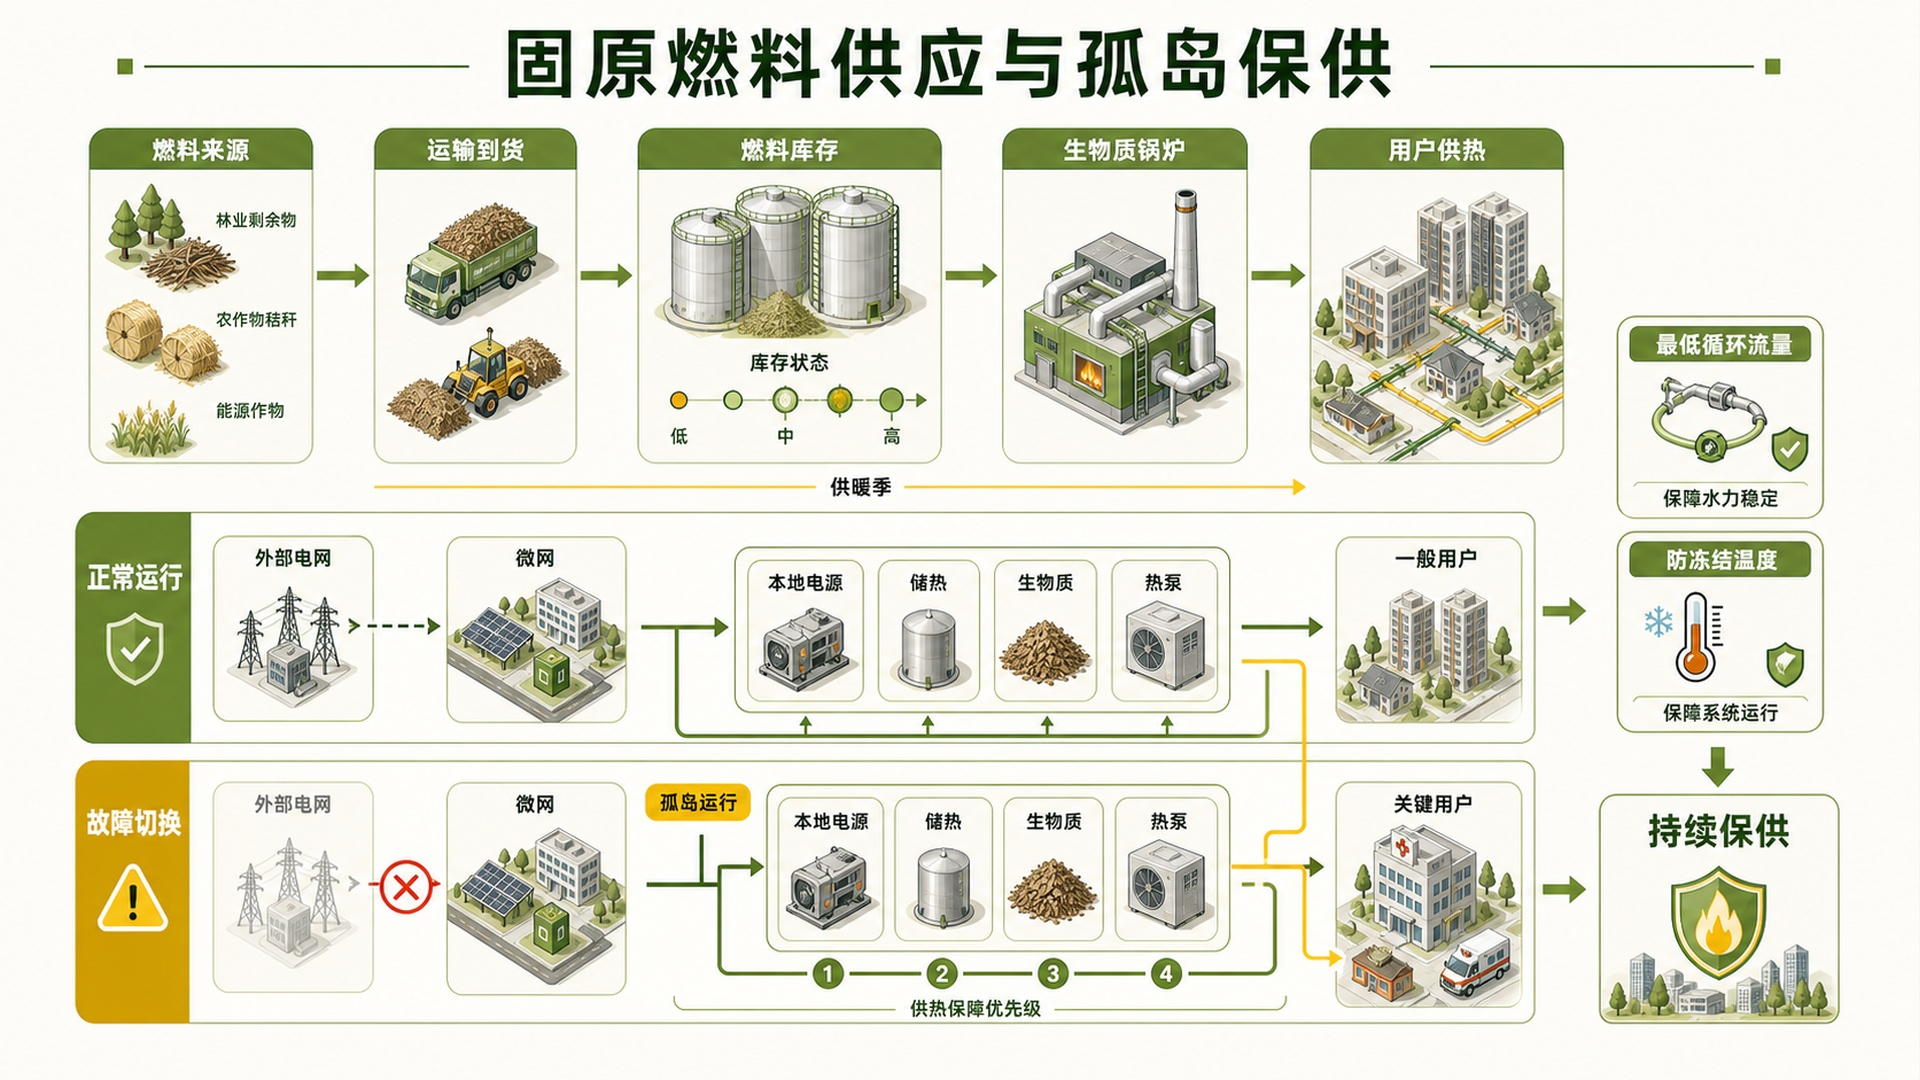
\includegraphics[width=0.76\textwidth,height=0.35\textheight,keepaspectratio]{media/model-cn/12_固原燃料与孤岛保供.jpg}
\caption{固原燃料与孤岛保供}
\label{fig:model-cn-guyuan-risk}
\end{figure}

\subsubsection{武汉场景}

武汉以楼栋和小区为主要空间单元。原框架用下式表达独立楼宇、区域能源站、低温热网和第五代区域供热供冷系统的形态选择接口；已报告算例按给定形态装配设备与运行约束：
\begin{equation}
z_i^{\mathrm{building}}+z_i^{\mathrm{station}}+z_i^{\mathrm{LTN}}+z_i^{\mathrm{5GDHC}}=1.
\end{equation}
四类形态的适用边界见图\ref{fig:model-cn-wuhan-types}。

\begin{figure}[H]
\centering
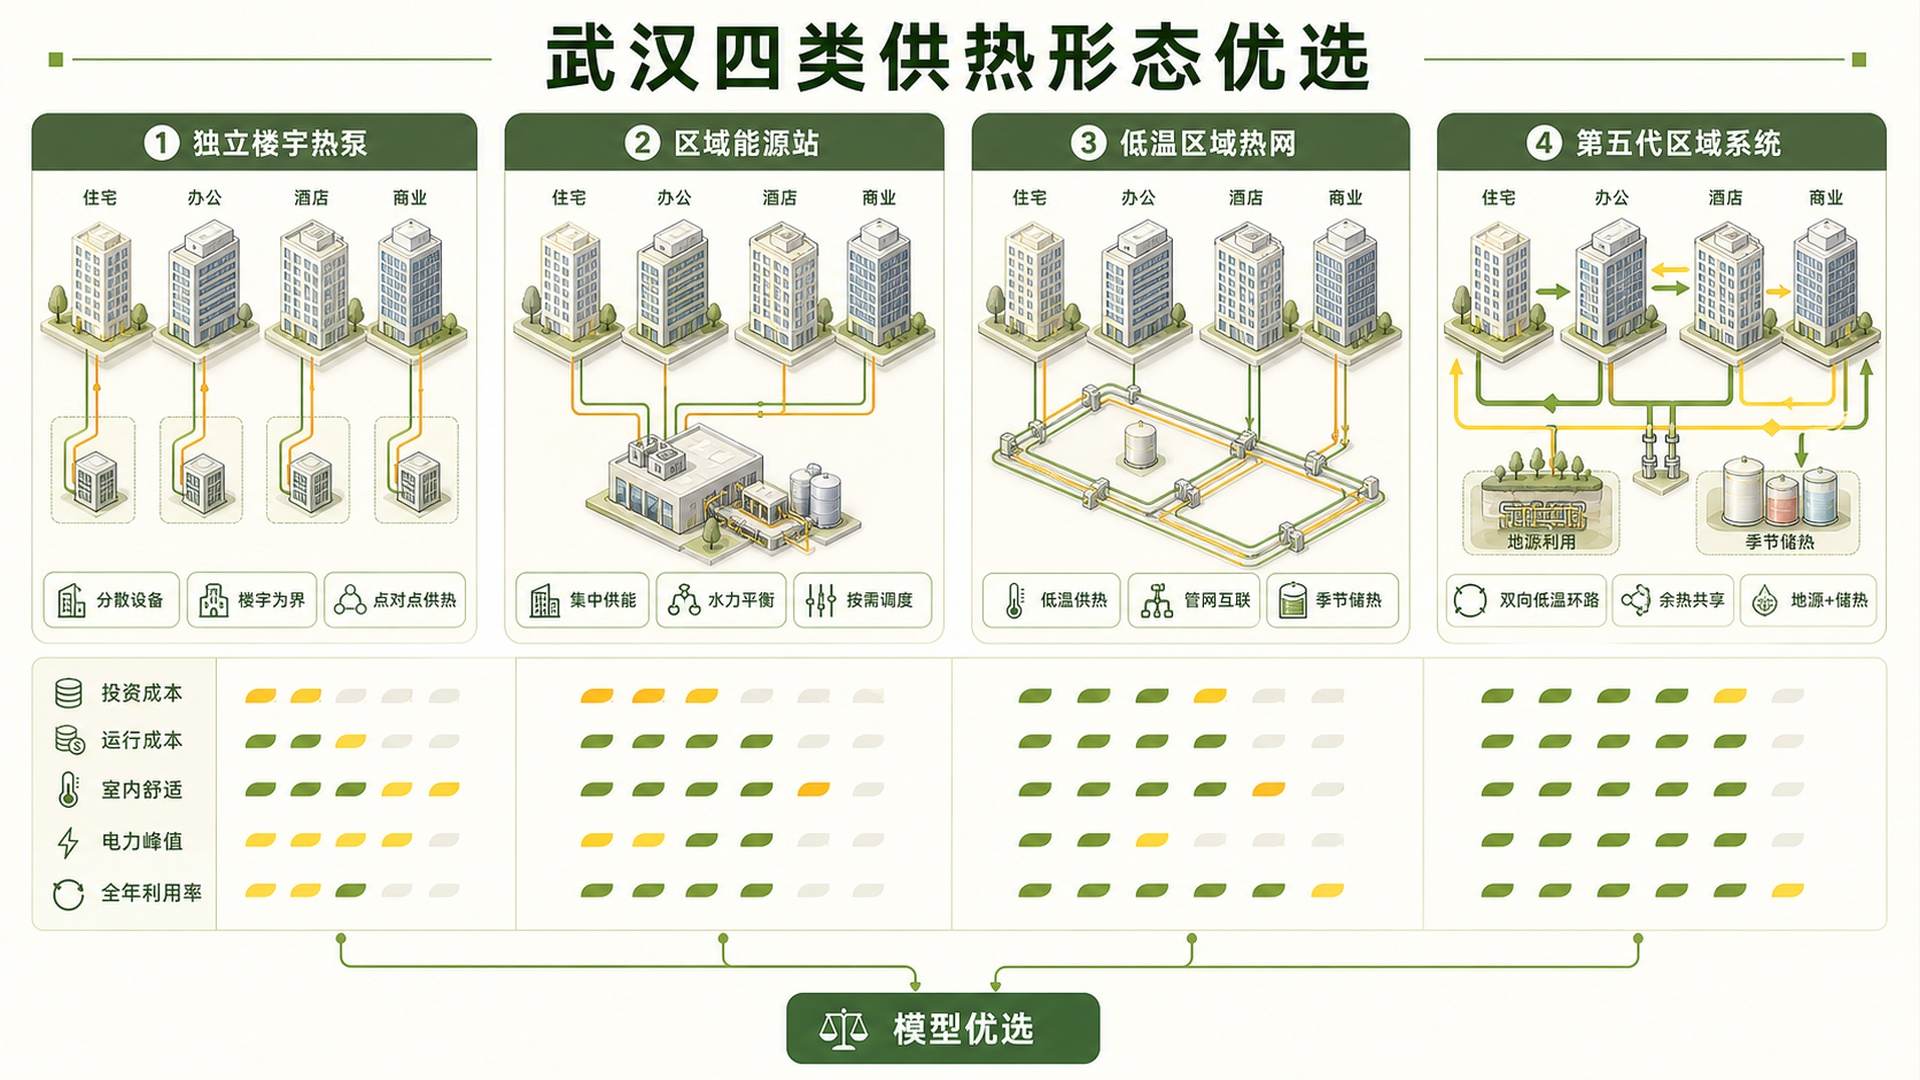
\includegraphics[width=0.76\textwidth,height=0.35\textheight,keepaspectratio]{media/model-cn/13_武汉四类供热形态.jpg}
\caption{武汉供热形态}
\label{fig:model-cn-wuhan-types}
\end{figure}

武汉场景重点考虑供热、间歇预热和楼栋配电容量，供冷与生活热水按配置启用；温湿度、新风、结露、除霜、地源年度平衡与噪声保留为扩展约束。其中，启用结露检查时，低温末端表面温度应高于露点并保留安全裕度：
\begin{equation}
T_{b,t}^{\mathrm{surface}}\geq T_{b,t}^{\mathrm{dew}}+\Delta T^{\mathrm{safe}}.
\end{equation}
主要约束见图\ref{fig:model-cn-wuhan-quality}，详细表达列于附录1。

逐楼舒适边界按占用时段配置，预热受热容、散热、设备与配电共同限制；恢复室温由状态递推获得。

\begin{figure}[H]
\centering
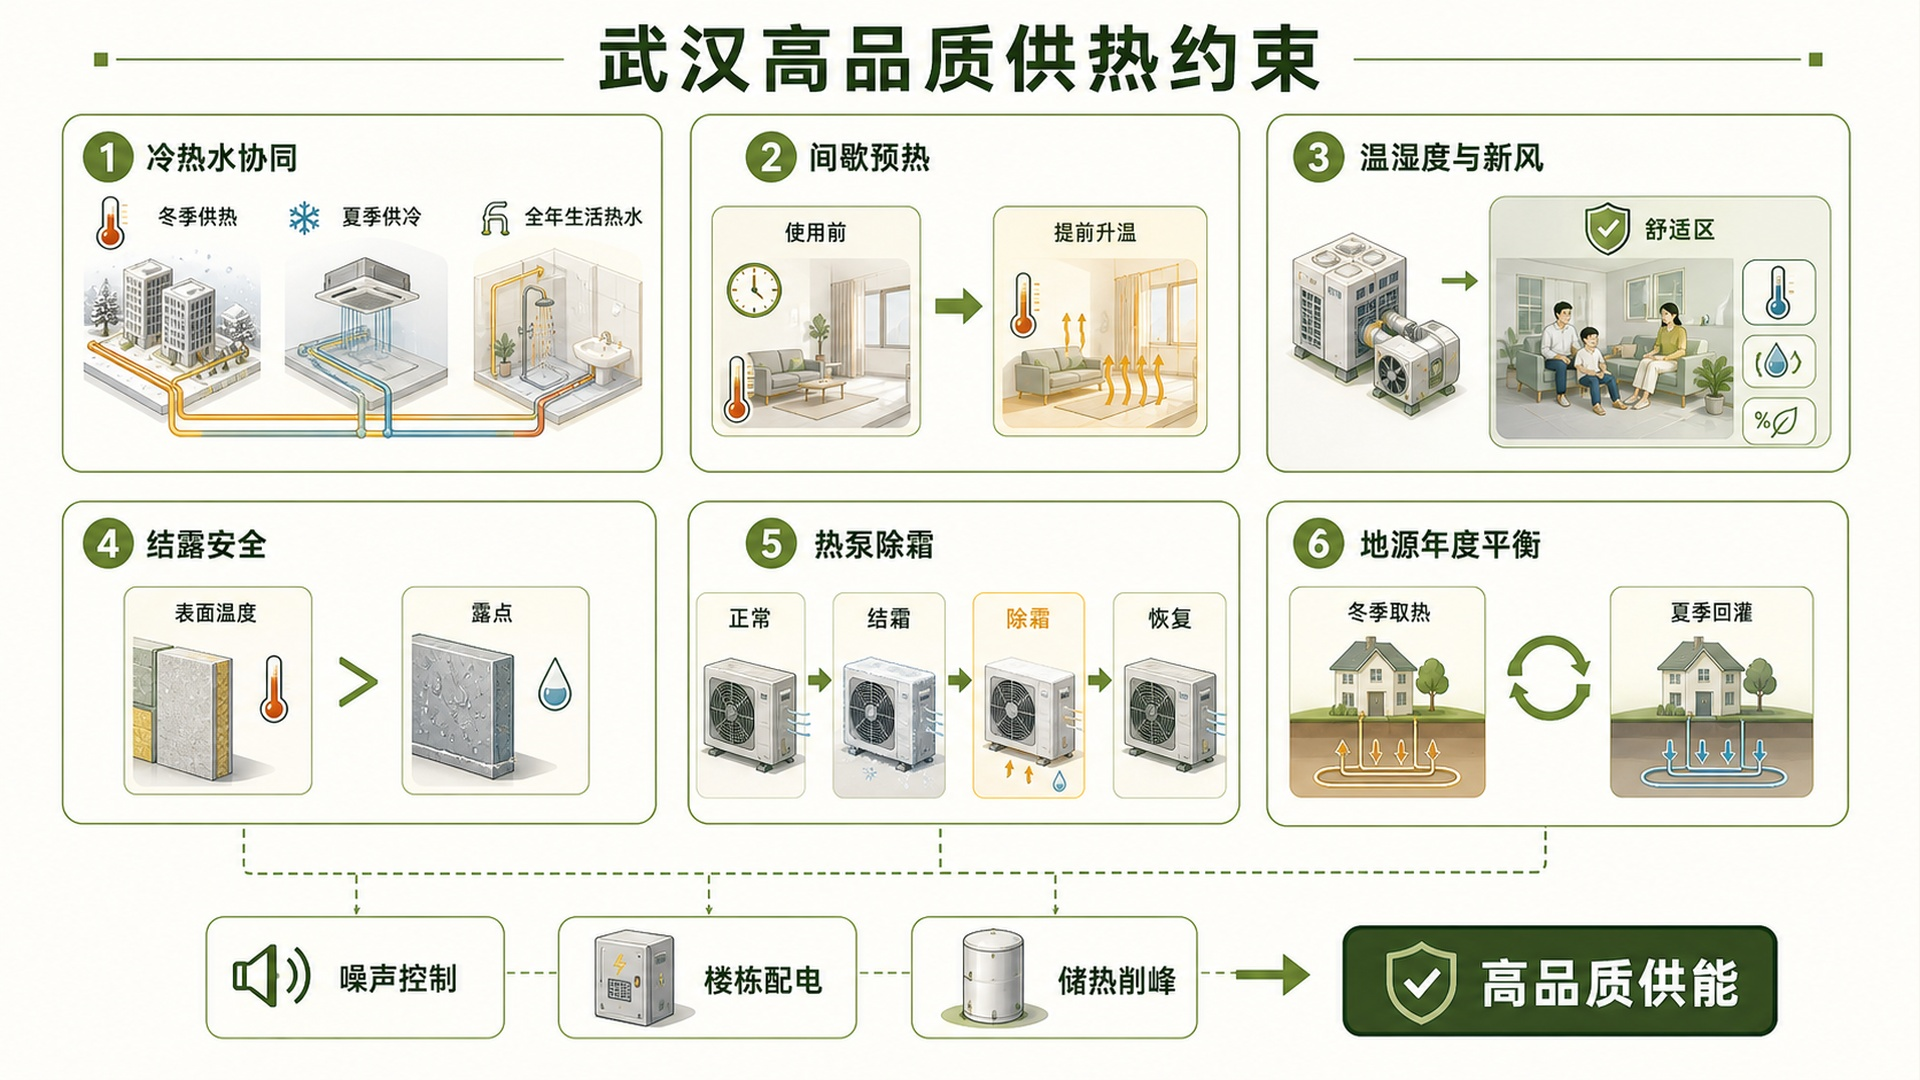
\includegraphics[width=0.76\textwidth,height=0.35\textheight,keepaspectratio]{media/model-cn/14_武汉高品质供热约束.jpg}
\caption{武汉供热约束}
\label{fig:model-cn-wuhan-quality}
\end{figure}

\subsection{场景差异}

三类场景共享负荷预测、能量平衡、容量演化、储热递推和舒适度约束，但规划对象和主导边界不同。乌鲁木齐侧重存量资产重构与极寒保供，固原侧重空间选址、燃料供应和微网可靠性，武汉侧重系统形态与多服务品质。共核与差异关系见图\ref{fig:model-cn-adapters}。

表中包含扩展边界，实际启用项见配置矩阵；同城按相同服务范围比较，跨城统一单位指标。

\begin{figure}[H]
\centering
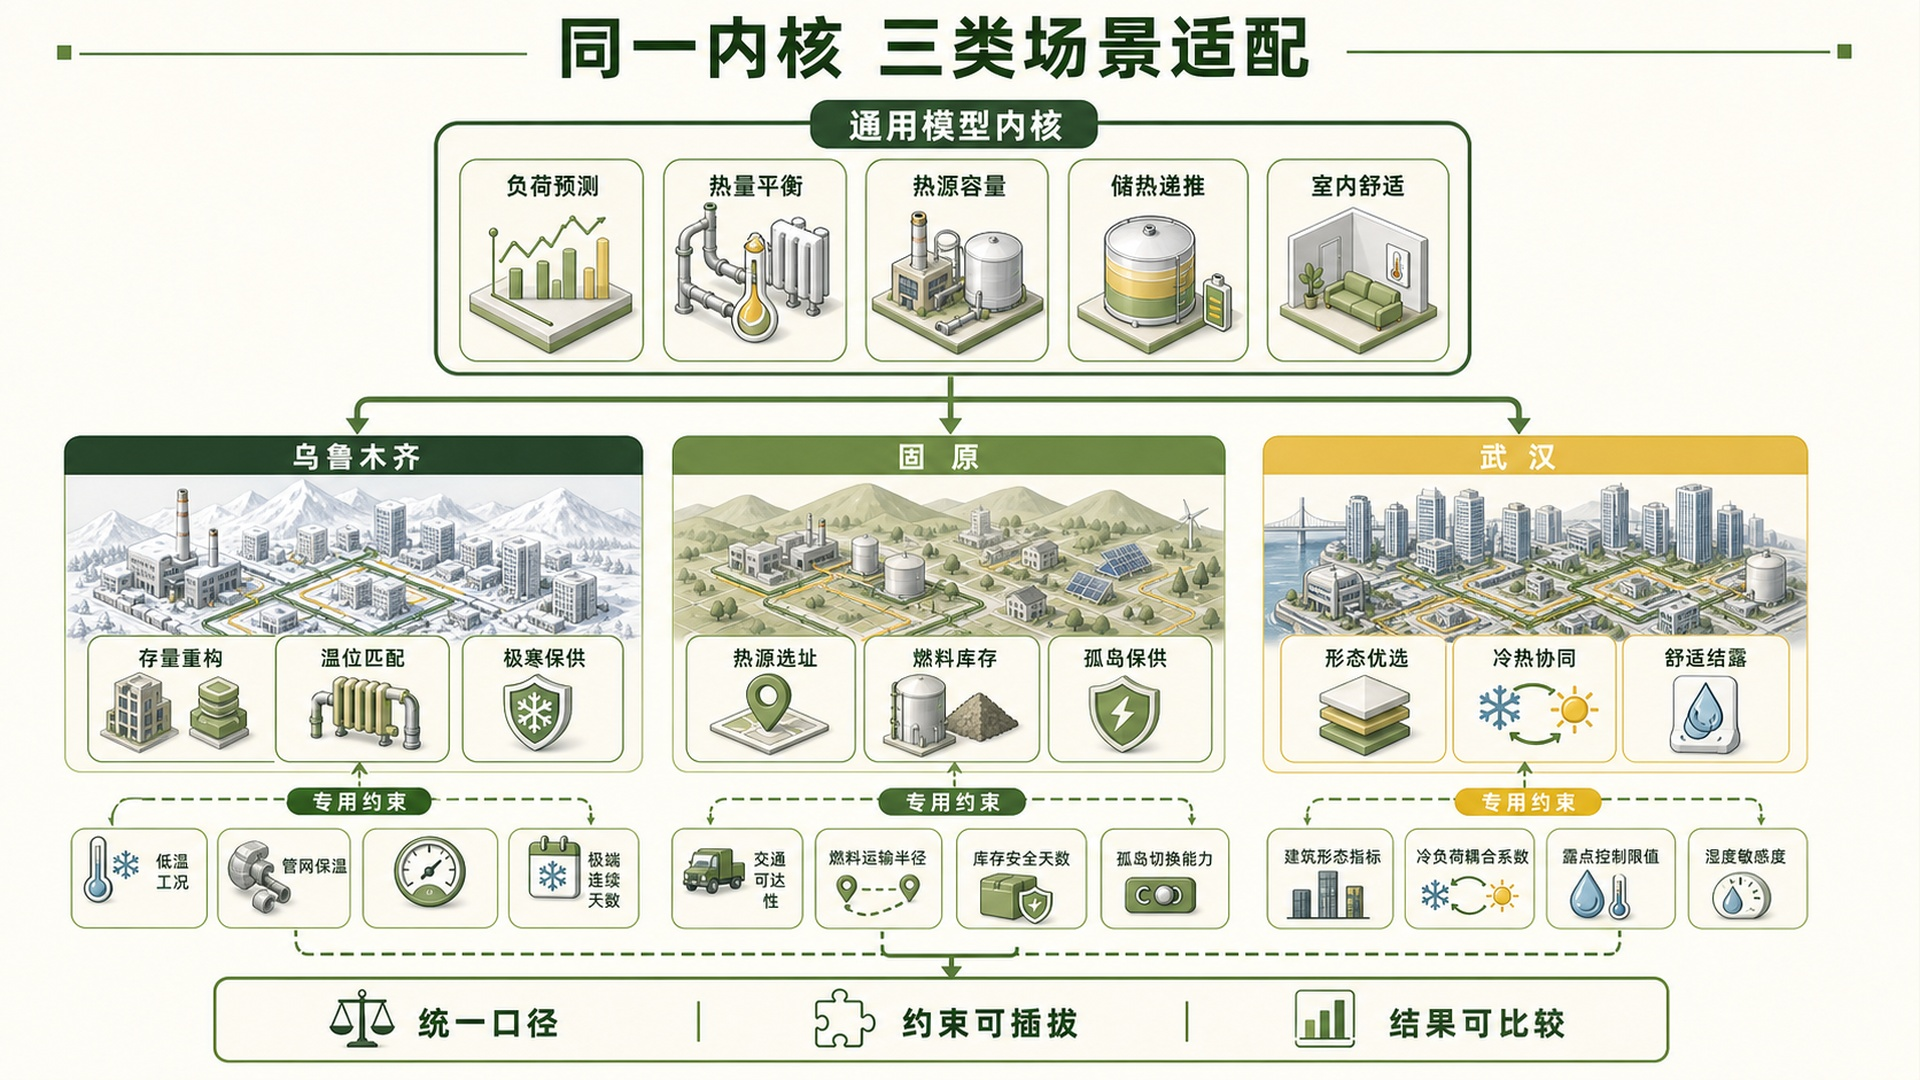
\includegraphics[width=0.76\textwidth,height=0.36\textheight,keepaspectratio]{media/model-cn/15_三城市共核异构.jpg}
\caption{三城市场景适配}
\label{fig:model-cn-adapters}
\end{figure}

\begin{table}[H]
\centering
\caption{三类场景的模型差异}
\small
\begin{tabularx}{\textwidth}{@{}L{0.13\textwidth}YYY@{}}
\toprule
维度 & 乌鲁木齐 & 固原 & 武汉\\
\midrule
初始条件 & 既有热源、骨干网和换热站 & 管网覆盖不足、分散热源较多 & 无传统集中供热资产\\
主要决策 & 热源退役、余热接入、管网降温 & 选址、用户分配、微网与燃料供应 & 供热形态、冷热水协同与配电\\
主导约束 & 温位、骨干网、N-1与寒潮保供 & 服务半径、库存、孤岛与防冻结 & 舒适、新风、结露、除霜与噪声\\
校核重点 & 远端温度、流量和回水温度 & 燃料到货、连通性和关键用户 & 温度恢复、地源平衡和配电容量\\
\bottomrule
\end{tabularx}
\end{table}

\subsection{统一校核}

三类场景采用相同的基础验收口径：逐时热量平衡残差不超过$\varepsilon_Q$，储热状态残差不超过$\varepsilon_E$，用户热状态满足边界，管网流量利用率不超过1，购电功率不超过接入容量，正常工况和规定压力情景下失供率为0；逐楼验证另检查室温舒适区间。统一指标与场景专用指标的对应关系见图\ref{fig:model-cn-acceptance}。

\begin{figure}[H]
\centering
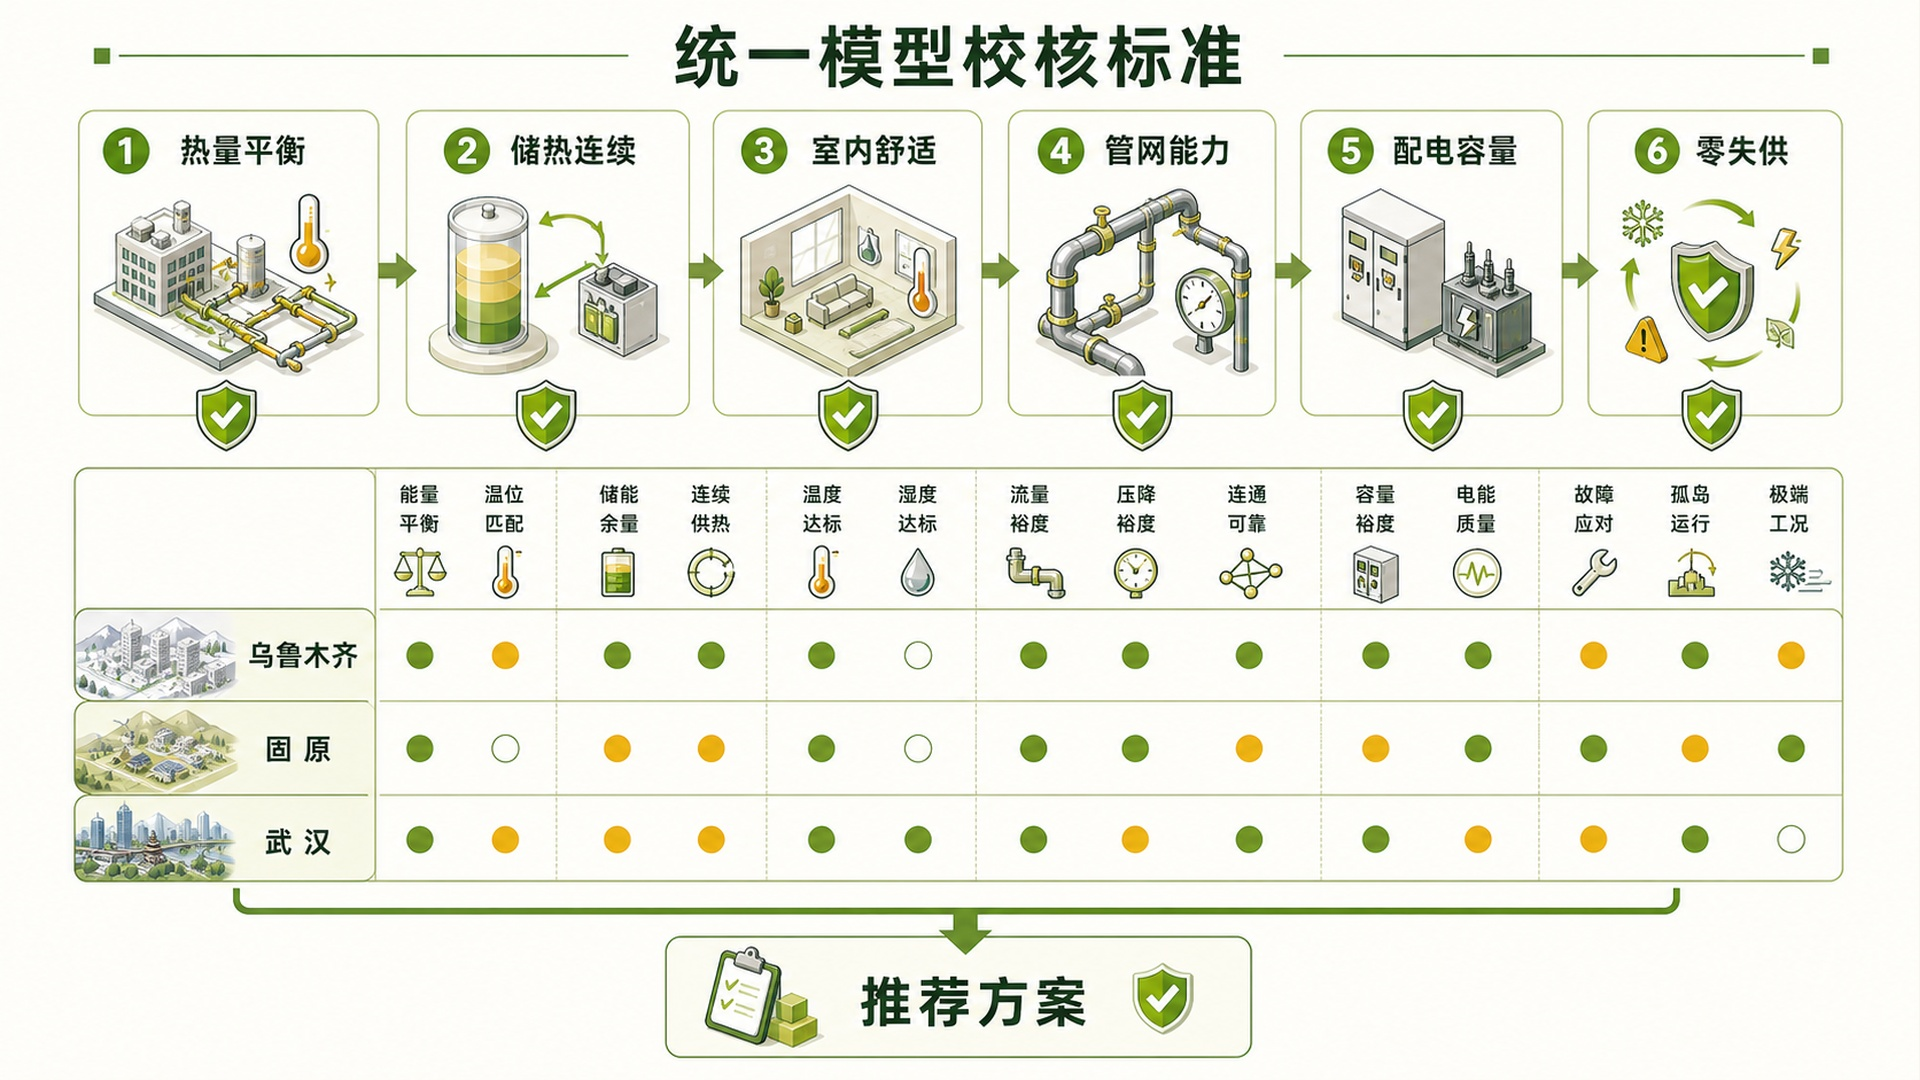
\includegraphics[width=0.62\textwidth,height=0.30\textheight,keepaspectratio]{media/model-cn/16_统一模型校核标准.jpg}
\caption{统一模型校核指标}
\label{fig:model-cn-acceptance}
\end{figure}

上述模型为后续算法提供变量、目标函数和可行域。规划变量确定资产与容量，运行变量描述供暖季逐时状态，工程校核用于确认候选方案满足连续物理边界。

\textbf{全季检验保留小时顺序，建筑与储热状态不逐日重置。}逐时执行守恒及运行边界；典型日仅用于筛选。记录最大残差、超限小时与对象、初末状态和输入版本。聚合案例、逐楼热状态与有限管网反馈分别登记验证范围，结果见数据验证章节。
